%!TEX root = sigir2013site_clicks.tex
\section{Analysis and Results}\label{sec_results}
In this section, we present our simulations and discuss our findings from each.

\subsection{A Perfect World}
As a form of implicit relevance feedback, obtaining clickthrough data under ideal conditions - where the collected data are free from any form of noise or bias - is a highly unrealistic goal to aim for in a real-world scenario.

Despite this, data collected in an ideal environment does provide us with a better understanding of the maximum attainable performance improvements that clickthroughs can theoretically provide. As such, examining data collected in ideal conditions allowed us to answer the following operational questions.

\begin{enumerate}
	
	\item{\emph{What is the maximum performance attainable when clickthrough data are incorporated?}}
	
	\item{\emph{How fast can maximum performance be reached?}}
	
\end{enumerate}

We addressed these questions with a series of simulations run across all three devised models. For each model, we set $P(C|N)$ to a 0.0, and vary $P(C|R)$, using the values 0.25, 0.5, 0.75 and 1.0. These settings exhibited the aforementioned `ideal' conditions, ensuring that all clicks are only on relevant documents. We hypothesised that as the probability of clicking on relevant documents is decreased, the number of iterations required to reach a maximum performance threshold increased - but would converge at the same points. We also varied the depth, $d$, of the simulations, using values of 10, 20 and 30. This was to examine whether an increase in depth would yield an increase or decrease in performance.

For the promotion-only algorithm \textbf{P}, we also ran simulations over a range of $\alpha$ values, namely 0.05, 0.1, 0.25, 0.5, 0.75, 1.0 and 2.0. For the demotion algorithms \textbf{PD} and \textbf{PDE}, we selected a value for $\alpha$ that offered good performance for \textbf{P}. However, we varied $\beta$ using the same numerical range.

\subsubsection{Results}
When combining `perfect' clickthrough evidence, we observed performance improvements over our baseline system of some 265\%. For \textbf{P}, a MAP of 0.2774 was attained. For \textbf{PD} and \textbf{PD}, MAP values of 0.6727 and 0.3931 were obtained respectively.

%For promotion-only model \textbf{P}, the results in Table \ref{tbl:results_perfect_multiplicative} provide a summary of our findings. For \textbf{P}, the maximum attainable performance was identical when $\alpha > 0$. When $d=10$, MAP increased from 0.1842 to 0.2188. When $d=20$ and $d=30$, MAP increased even further - to 0.2358 and 0.2774 respectively. The explanation for this behaviour is that as $d$ increases, more documents in the document rankings have a chance to be promoted. $\alpha$, while having no effect on overall performance, does vary the rates at which performance converges. A higher $\alpha$ value results in performance converging in fewer iterations.

%\todo{==========}

\textbf{\emph{What is the maximum performance attainable when clickthrough data is incorporated?}}
Improvements over our baseline across all three clickthrough models. Running each model across our three chosen depths of 10, 20 and 30, we noted that performance increased further the greater the depth. This finding is intuitive, and can be explained by the fact that as the simulation depth increases, more potentially relevant documents will be viewed and clicked, which percolate up the rankings.

\begin{table}[t!]
	\renewcommand{\arraystretch}{1.3}
	\begin{center}
		\begin{small}
			\begin{tabularx}{\linewidth}{W{0.86cm}|W{1.4cm}|W{1.4cm}|W{1.4cm}|W{1.4cm}W{0.00000001cm}}
				
			 	& & \centering{\textbf{\emph{MAP}}} & \centering{\textbf{\emph{P@5}}} & \centering{\textbf{\emph{P@10}}}&
				\tabularnewline
				\hline
				
				\centering{BL}
				& \centering{$\alpha = 0$}
				& \centering{0.1842}
				& \centering{0.2720}
				& \centering{0.2260}&
				\tabularnewline[1em]
				\hline
				
				\multirow{4}{*}{\vspace{-2cm}\hspace{0.18cm}\begin{rotate}{90}$P(C|R) > 0.0$\end{rotate}}
				& \centering{$\alpha > 0$\\$d = 10$}
				& \centering{0.2188}
				& \centering{0.4240}
				& \centering{0.2260}&
				\tabularnewline
				\cline{2-5}
				
				& \centering{$\alpha > 0$\\$d = 20$}
				& \centering{0.2358}
				& \centering{0.5320}
				& \centering{0.3520}&
				\tabularnewline
				\cline{2-5}
				
				& \centering{$\alpha > 0$\\$d = 30$}
				& \centering{\textbf{0.2774}}
				& \centering{\textbf{0.5960}}
				& \centering{\textbf{0.4240}}&
				\tabularnewline
				
				
			\end{tabularx}
		\end{small}
	\end{center}
	
	\vspace{-0.4cm}
	\caption{\textbf{Table illustrating the highest performance levels attained using the promotion-only model. The table shows performance differences across varying simulation depths. \emph{BL} indicates baseline values.}\vspace{-0.2cm}}
	\label{tbl:results_perfect_multiplicative}
\end{table}

\begin{table}[t!]
	\renewcommand{\arraystretch}{1.3}
	\begin{center}
		\begin{small}
			\begin{tabularx}{\linewidth}{W{0.86cm}|W{1.4cm}|W{1.4cm}|W{1.4cm}|W{1.4cm}W{0.00000001cm}}
			 	& & \centering{\textbf{\emph{MAP}}} & \centering{\textbf{\emph{P@5}}} & \centering{\textbf{\emph{P@10}}} &
				\tabularnewline
				\hline
				
				\centering{BL}
				& \centering{$\alpha = 0$}
				& \centering{0.1842}
				& \centering{0.2720}
				& \centering{0.2260} &
				\tabularnewline[1em]
				\hline
				
				\hspace{4cm}P
				& \multicolumn{1}{c|}{\multirow{2}{*}{\begin{varwidth}{1.15cm}\centering{$\alpha=0.75$ $d=30$}\end{varwidth}}}
				& \centering{0.2774}
				& \centering{0.5960}
				& \centering{0.4240} &
				\tabularnewline[1.4em]
				\cline{3-5}
				
				&
				& \multicolumn{3}{c}{$i = 12$}
				\tabularnewline
				
				\hline
				\hline
				
				\multirow{4}{*}{\vspace{-3.45cm}\hspace{0.18cm}\begin{rotate}{90}$P(C|R) > 0.25$\end{rotate}}
				& \multicolumn{1}{c|}{\multirow{2}{*}{\begin{varwidth}{1.15cm}\centering{$\alpha=0.75$ $\beta>0$ $d=10$}\end{varwidth}}}
				& \centering{{\makebox[0pt][c]{{\tiny $\beta@0.05$} 0.4412}\\\makebox[0pt][c]{{\tiny $\beta@2.0$} 0.5140}}}
				& \centering{{\makebox[0pt][c]{{\tiny $\beta@0.05$} 0.8720}\\\makebox[0pt][c]{{\tiny $\beta@2.0$} 0.7160}}}
				& \centering{{\makebox[0pt][c]{{\tiny $\beta@0.05$} 0.8920}\\\makebox[0pt][c]{{\tiny $\beta@2.0$} 0.8100}}} &
				\tabularnewline[1.4em]
				\cline{3-5}
				
				&
				& \multicolumn{3}{c}{$\beta = 0.05, i = 1000$ - $\beta = 2.00, i = 685$}
				\tabularnewline
				\cline{2-5}
				
				& \multicolumn{1}{c|}{\multirow{2}{*}{\begin{varwidth}{1.15cm}\centering{$\alpha=0.75$ $\beta>0$ $d=20$}\end{varwidth}}}
				& \centering{{\makebox[0pt][c]{{\tiny $\beta@0.05$} 0.5732}\\\makebox[0pt][c]{{\tiny $\beta@2.0$} 0.6318}}}
				& \centering{{\makebox[0pt][c]{{\tiny $\beta@0.05$} 0.8880}\\\makebox[0pt][c]{{\tiny $\beta@2.0$} 0.8920}}}
				& \centering{{\makebox[0pt][c]{{\tiny $\beta@0.05$} 0.7940}\\\makebox[0pt][c]{{\tiny $\beta@2.0$} 0.8100}}} &
				\tabularnewline[1.4em]
				\cline{3-5}
				
				&
				& \multicolumn{3}{c}{$\beta = 0.05, i = 1000$ - $\beta = 2.00, i = 381$}
				\tabularnewline
				\cline{2-5}
				
				& \multicolumn{1}{c|}{\multirow{2}{*}{\begin{varwidth}{1.15cm}\centering{$\alpha=0.75$ $\beta>0$ $d=30$}\end{varwidth}}}
				& \centering{{\makebox[0pt][c]{{\tiny $\beta@0.05$} 0.6269}\\\makebox[0pt][c]{{\tiny $\beta@2.0$} 0.6727}}}
				& \centering{{\makebox[0pt][c]{{\tiny $\beta@0.05$} 0.8920}\\\makebox[0pt][c]{{\tiny $\beta@2.0$} 0.8920}}}
				& \centering{{\makebox[0pt][c]{{\tiny $\beta@0.05$} 0.8060}\\\makebox[0pt][c]{{\tiny $\beta@2.0$} 0.8100}}} &
				\tabularnewline[1.4em]
				\cline{3-5}
				
				&
				& \multicolumn{3}{c}{$\beta = 0.05, i = 995$ - $\beta = 2.00, i = 311$}
				\tabularnewline
				\hline
				\hline
				
				\multirow{4}{*}{\vspace{-3.45cm}\hspace{0.18cm}\begin{rotate}{90}$P(C|R) = 0.25$\end{rotate}}
				& \multicolumn{1}{c|}{\multirow{2}{*}{\begin{varwidth}{1.15cm}\centering{$\alpha=0.75$ $\beta>0$ $d=10$}\end{varwidth}}}
				& \centering{{\makebox[0pt][c]{{\tiny $\beta@0.05$} 0.4333}\\\makebox[0pt][c]{{\tiny $\beta@2.0$} 0.1842}}}
				& \centering{{\makebox[0pt][c]{{\tiny $\beta@0.05$} 0.8600}\\\makebox[0pt][c]{{\tiny $\beta@2.0$} 0.2720}}}
				& \centering{{\makebox[0pt][c]{{\tiny $\beta@0.05$} 0.7040}\\\makebox[0pt][c]{{\tiny $\beta@2.0$} 0.2260}}} &
				\tabularnewline[1.4em]
				\cline{3-5}
				
				&
				& \multicolumn{3}{c}{$\beta = 0.05, i = 992$ - $\beta = 2.00, i = 0$}
				\tabularnewline
				\cline{2-5}
				
				& \multicolumn{1}{c|}{\multirow{2}{*}{\begin{varwidth}{1.15cm}\centering{$\alpha=0.75$ $\beta>0$ $d=20$}\end{varwidth}}}
				& \centering{{\makebox[0pt][c]{{\tiny $\beta@0.05$} 0.5668}\\\makebox[0pt][c]{{\tiny $\beta@2.0$} 0.1842}}}
				& \centering{{\makebox[0pt][c]{{\tiny $\beta@0.05$} 0.8880}\\\makebox[0pt][c]{{\tiny $\beta@2.0$} 0.2720}}}
				& \centering{{\makebox[0pt][c]{{\tiny $\beta@0.05$} 0.7840}\\\makebox[0pt][c]{{\tiny $\beta@2.0$} 0.2260}}} &
				\tabularnewline[1.4em]
				\cline{3-5}
				
				&
				& \multicolumn{3}{c}{$\beta = 0.05, i = 1000$ - $\beta = 2.00, i = 0$}
				\tabularnewline
				\cline{2-5}
				
				& \multicolumn{1}{c|}{\multirow{2}{*}{\begin{varwidth}{1.15cm}\centering{$\alpha=0.75$ $\beta>0$ $d=30$}\end{varwidth}}}
				& \centering{{\makebox[0pt][c]{{\tiny $\beta@0.05$} 0.6243}\\\makebox[0pt][c]{{\tiny $\beta@2.0$} 0.1842}}}
				& \centering{{\makebox[0pt][c]{{\tiny $\beta@0.05$} 0.8920}\\\makebox[0pt][c]{{\tiny $\beta@2.0$} 0.2720}}}
				& \centering{{\makebox[0pt][c]{{\tiny $\beta@0.05$} 0.8060}\\\makebox[0pt][c]{{\tiny $\beta@2.0$} 0.2260}}} &
				\tabularnewline[1.4em]
				\cline{3-5}
				
				&
				& \multicolumn{3}{c}{$\beta = 0.05, i = 1000$ - $\beta = 2.00, i = 0$}
				\tabularnewline
				
			\end{tabularx}
		\end{small}
	\end{center}
	
	\vspace{-0.4cm}
	\caption{\textbf{Table summarising the performance values achieved across varying $P(C|R)$ and depth values using the \emph{PD} model, where $\alpha = 0.75$. For brevity, very similar results for $P(C|R) = 0.25$, $P(C|R) = 0.5$ and $P(C|R) = 0.75$ are condensed into $P(C|R) > 0.25$. \emph{BL} indicates baseline values, \textbf{\emph{P}} denotes the best performance achieved using model \emph{P}. Lower $i$ values indicate maximum performance is reached earlier.}\vspace{-0.4cm}}
	\label{tbl:results_perfect_demotive}
\end{table}

Starting with our baseline MAP of 0.1842, our three models improved to maximums of 0.2774, 0.6727 and 0.3931 for models \textbf{P}, \textbf{PD} and \textbf{PDE} respectively - with all values being observed with $d=30$. Tables \ref{tbl:results_perfect_multiplicative}, \ref{tbl:results_perfect_demotive} and \ref{tbl:results_perfect_view} present the maximum performance values obtained across the parameters we varied. To obtain the best performance, it did not matter what value $\alpha$ was assigned. We decided to use $\alpha = 0.75$ for the other two models so as to not dominate their respective demotion aspects.

Of interest is the varying performance levels observed between the three models. With the performance of \textbf{PD} clearly superior to \textbf{P} and \textbf{PDE}, what are the key differences between the models which can account for such a variation?

Compared to \textbf{PD}, model \textbf{P} is promotion-only, meaning that irrelevant documents are not directly demoted. They may however fall down rankings as relevant documents are pushed up, but never at the same rate as a promotion and demotion approach. Model \textbf{PDE} -  while possessing the ability to demote documents - also takes into account the rank at which documents reside. This means that documents at lower ranks are less likely to be promoted, explaining the difference in performance over model \textbf{PD}.

Also important to achieving a high performance is the value of demotion tuning parameter, $\beta$. Too high, the demotion aspect of \textbf{PD} and \textbf{PDE} becomes too aggressive; too low, the demotion aspect is not aggressive enough. By examining Tables \ref{tbl:results_perfect_demotive} and \ref{tbl:results_perfect_view}, it can be seen that the best performance is achieved when $\beta = 2.0$. However, as $P(C|R)$ is decreased, the best performance can be attained with a much smaller $\beta$ value. This can be explained due to the fact that with a lower $P(C|R)$ value, relevant documents are less likely to be clicked. With fewer clicks, documents are more susceptible to demotion.

To examine this phenomenon, we ran a further simulation using \textbf{PD} and set $P(C|R)$ to 0.25. We varied $\beta$ from 0.0 to 2.0. We used steps of 0.01 between 0.0 and 0.25 to obtain a better perspective of performance at lower $\beta$ values.  As shown in Figure \ref{fig:perfect_map_fall}, results show a peak in performance at much lower $\beta$ values - in the range from 0.05 to 0.20. After 0.20, performance begins to drop significantly as the demotion aspect of the \textbf{PD} model becomes too aggressive. In some cases, demotion is so aggressive that performance begins to drop - in some cases \emph{below} our baseline values.
 
\begin{figure}
	\begin{center}
	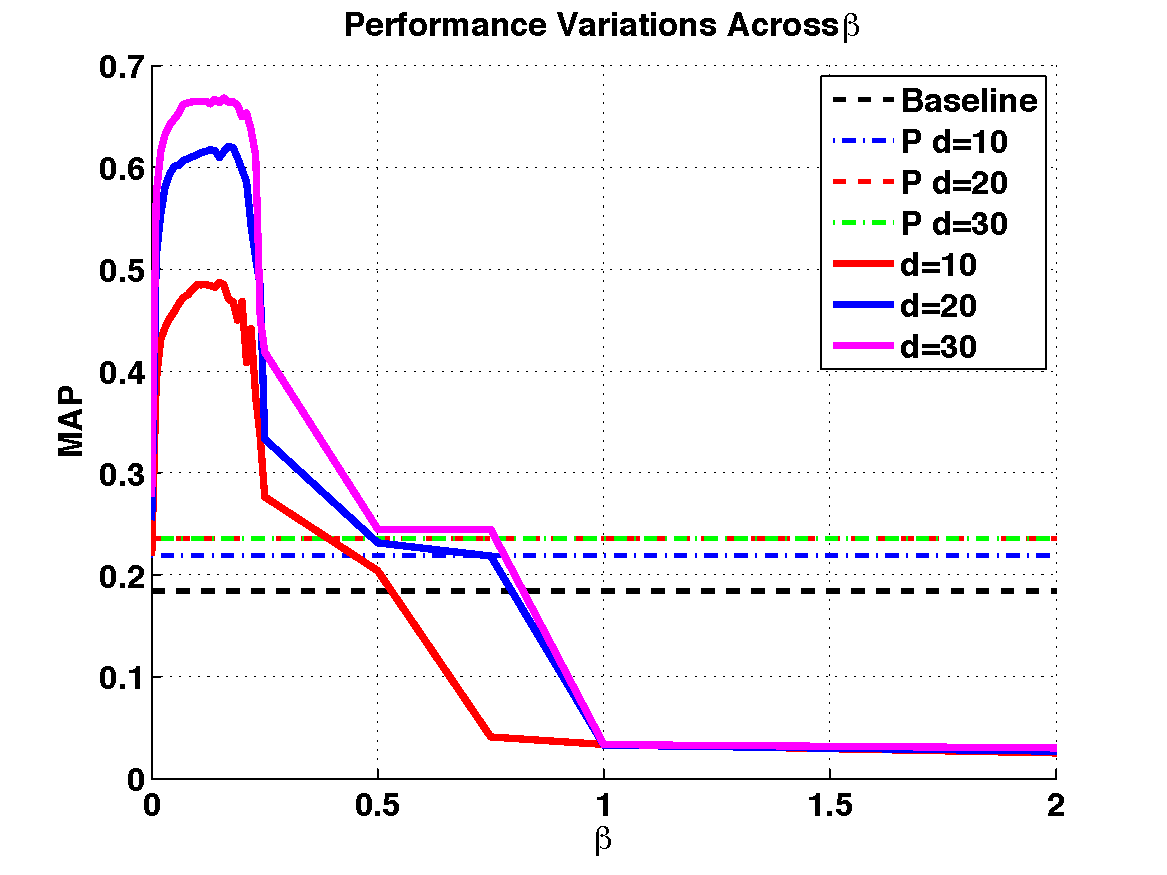
\includegraphics[width=\linewidth]{pics/perfect/perfect_map_fall.pdf}
	\end{center}
	\vspace{-0.5cm}
	\caption{\label{fig:perfect_map_fall}\textbf{A line graph illustrating the significant fall in performance as $\beta$ is increased after 0.25. Data are from the `ideal' simulations for the PD model with $P(C|R) = 0.25$.}\vspace{-0.5cm}}
\end{figure}

\textbf{\emph{How fast can maximum performance be reached?}}
The number of iterations required for performance to reach its maximum varies on a combination of parameters. We varied $P(C|R)$ to specifically examine this issue. For many cases where performance continues to increase with a lower $P(C|R)$ value, several simulations hit our imposed limit of 1000 iterations; we hypothesise that if these were to continue, performance would eventually converge.

\begin{table}[t!]
	\renewcommand{\arraystretch}{1.3}
	\begin{center}
		\begin{small}
			\begin{tabularx}{\linewidth}{W{0.86cm}|W{1.4cm}|W{1.4cm}|W{1.4cm}|W{1.4cm}W{0.00000001cm}}
			 	& & \centering{\textbf{\emph{MAP}}} & \centering{\textbf{\emph{P@5}}} & \centering{\textbf{\emph{P@10}}} &
				\tabularnewline
				\hline
				
				\centering{BL}
				& \centering{$\alpha = 0$}
				& \centering{0.1842}
				& \centering{0.2720}
				& \centering{0.2260} &
				\tabularnewline[1em]
				\hline
				
				\hspace{4cm}P
				& \multicolumn{1}{c|}{\multirow{2}{*}{\begin{varwidth}{1.15cm}\centering{$\alpha=0.75$ $d=30$}\end{varwidth}}}
				& \centering{0.2774}
				& \centering{0.5960}
				& \centering{0.4240} &
				\tabularnewline[1.4em]
				\cline{3-5}
				
				&
				& \multicolumn{3}{c}{$i = 12$}
				\tabularnewline
				
				\hline
				\hline
				
				\multirow{4}{*}{\vspace{-3.45cm}\hspace{0.18cm}\begin{rotate}{90}$P(C|R) = 1.0$\end{rotate}}
				& \multicolumn{1}{c|}{\multirow{2}{*}{\begin{varwidth}{1.15cm}\centering{$\alpha=0.75$ $\beta>0$ $d=10$}\end{varwidth}}}
				& \centering{{\makebox[0pt][c]{{\tiny $\beta@0.05$} 0.2592}\\\makebox[0pt][c]{{\tiny $\beta@2.0$} 0.2869}}}
				& \centering{{\makebox[0pt][c]{{\tiny $\beta@0.05$} 0.5600}\\\makebox[0pt][c]{{\tiny $\beta@2.0$} 0.6520}}}
				& \centering{{\makebox[0pt][c]{{\tiny $\beta@0.05$} 0.3420}\\\makebox[0pt][c]{{\tiny $\beta@2.0$} 0.4320}}} &
				\tabularnewline[1.4em]
				\cline{3-5}
				
				&
				& \multicolumn{3}{c}{$\beta = 0.05, i = 993$ - $\beta = 2.00, i = 1000$}
				\tabularnewline
				\cline{2-5}
				
				& \multicolumn{1}{c|}{\multirow{2}{*}{\begin{varwidth}{1.15cm}\centering{$\alpha=0.75$ $\beta>0$ $d=20$}\end{varwidth}}}
				& \centering{{\makebox[0pt][c]{{\tiny $\beta@0.05$} 0.3068}\\\makebox[0pt][c]{{\tiny $\beta@2.0$} 0.3514}}}
				& \centering{{\makebox[0pt][c]{{\tiny $\beta@0.05$} 0.6560}\\\makebox[0pt][c]{{\tiny $\beta@2.0$} 0.7280}}}
				& \centering{{\makebox[0pt][c]{{\tiny $\beta@0.05$} 0.4720}\\\makebox[0pt][c]{{\tiny $\beta@2.0$} 0.5440}}} &
				\tabularnewline[1.4em]
				\cline{3-5}
				
				&
				& \multicolumn{3}{c}{$\beta = 0.05, i = 974$ - $\beta = 2.00, i = 998$}
				\tabularnewline
				\cline{2-5}
				
				& \multicolumn{1}{c|}{\multirow{2}{*}{\begin{varwidth}{1.15cm}\centering{$\alpha=0.75$ $\beta>0$ $d=30$}\end{varwidth}}}
				& \centering{{\makebox[0pt][c]{{\tiny $\beta@0.05$} 0.3383}\\\makebox[0pt][c]{{\tiny $\beta@2.0$} 0.3927}}}
				& \centering{{\makebox[0pt][c]{{\tiny $\beta@0.05$} 0.6960}\\\makebox[0pt][c]{{\tiny $\beta@2.0$} 0.7520}}}
				& \centering{{\makebox[0pt][c]{{\tiny $\beta@0.05$} 0.5180}\\\makebox[0pt][c]{{\tiny $\beta@2.0$} 0.5920}}} &
				\tabularnewline[1.4em]
				\cline{3-5}
				
				&
				& \multicolumn{3}{c}{$\beta = 0.05, i = 1000$ - $\beta = 2.00, i = 1000$}
				\tabularnewline
				\hline
				\hline
				
				\multirow{4}{*}{\vspace{-3.45cm}\hspace{0.18cm}\begin{rotate}{90}$P(C|R) = 0.75$\end{rotate}}
				& \multicolumn{1}{c|}{\multirow{2}{*}{\begin{varwidth}{1.15cm}\centering{$\alpha=0.75$ $\beta>0$ $d=10$}\end{varwidth}}}
				& \centering{{\makebox[0pt][c]{{\tiny $\beta@0.05$} 0.2592}\\\makebox[0pt][c]{{\tiny $\beta@2.0$} 0.2857}}}
				& \centering{{\makebox[0pt][c]{{\tiny $\beta@0.05$} 0.5600}\\\makebox[0pt][c]{{\tiny $\beta@2.0$} 0.6400}}}
				& \centering{{\makebox[0pt][c]{{\tiny $\beta@0.05$} 0.3420}\\\makebox[0pt][c]{{\tiny $\beta@2.0$} 0.4220}}} &
				\tabularnewline[1.4em]
				\cline{3-5}
				
				&
				& \multicolumn{3}{c}{$\beta = 0.05, i = 988$ - $\beta = 2.00, i = 1000$}
				\tabularnewline
				\cline{2-5}
				
				& \multicolumn{1}{c|}{\multirow{2}{*}{\begin{varwidth}{1.15cm}\centering{$\alpha=0.75$ $\beta>0$ $d=20$}\end{varwidth}}}
				& \centering{{\makebox[0pt][c]{{\tiny $\beta@0.05$} 0.3068}\\\makebox[0pt][c]{{\tiny $\beta@2.0$} 0.3494}}}
				& \centering{{\makebox[0pt][c]{{\tiny $\beta@0.05$} 0.6560}\\\makebox[0pt][c]{{\tiny $\beta@2.0$} 0.7200}}}
				& \centering{{\makebox[0pt][c]{{\tiny $\beta@0.05$} 0.4720}\\\makebox[0pt][c]{{\tiny $\beta@2.0$} 0.5400}}} &
				\tabularnewline[1.4em]
				\cline{3-5}
				
				&
				& \multicolumn{3}{c}{$\beta = 0.05, i = 968$ - $\beta = 2.00, i = 1000$}
				\tabularnewline
				\cline{2-5}
				
				& \multicolumn{1}{c|}{\multirow{2}{*}{\begin{varwidth}{1.15cm}\centering{$\alpha=0.75$ $\beta>0$ $d=30$}\end{varwidth}}}
				& \centering{{\makebox[0pt][c]{{\tiny $\beta@0.05$} 0.3371}\\\makebox[0pt][c]{{\tiny $\beta@2.0$} 0.3931}}}
				& \centering{{\makebox[0pt][c]{{\tiny $\beta@0.05$} 0.6920}\\\makebox[0pt][c]{{\tiny $\beta@2.0$} 0.7520}}}
				& \centering{{\makebox[0pt][c]{{\tiny $\beta@0.05$} 0.5140}\\\makebox[0pt][c]{{\tiny $\beta@2.0$} 0.5920}}} &
				\tabularnewline[1.4em]
				\cline{3-5}
				
				&
				& \multicolumn{3}{c}{$\beta = 0.05, i = 1000$ - $\beta = 2.00, i = 1000$}
				\tabularnewline
				\hline
				\hline
				
				\multirow{4}{*}{\vspace{-3.45cm}\hspace{0.18cm}\begin{rotate}{90}$P(C|R) = 0.5$\end{rotate}}
				& \multicolumn{1}{c|}{\multirow{2}{*}{\begin{varwidth}{1.15cm}\centering{$\alpha=0.75$ $\beta>0$ $d=10$}\end{varwidth}}}
				& \centering{{\makebox[0pt][c]{{\tiny $\beta@0.05$} 0.2592}\\\makebox[0pt][c]{{\tiny $\beta@2.0$} 0.2052}}}
				& \centering{{\makebox[0pt][c]{{\tiny $\beta@0.05$} 0.5600}\\\makebox[0pt][c]{{\tiny $\beta@2.0$} 0.4200}}}
				& \centering{{\makebox[0pt][c]{{\tiny $\beta@0.05$} 0.3440}\\\makebox[0pt][c]{{\tiny $\beta@2.0$} 0.2480}}} &
				\tabularnewline[1.4em]
				\cline{3-5}
				
				&
				& \multicolumn{3}{c}{$\beta = 0.05, i = 1000$ - $\beta = 2.00, i = 15$}
				\tabularnewline
				\cline{2-5}
				
				& \multicolumn{1}{c|}{\multirow{2}{*}{\begin{varwidth}{1.15cm}\centering{$\alpha=0.75$ $\beta>0$ $d=20$}\end{varwidth}}}
				& \centering{{\makebox[0pt][c]{{\tiny $\beta@0.05$} 0.3069}\\\makebox[0pt][c]{{\tiny $\beta@2.0$} 0.2631}}}
				& \centering{{\makebox[0pt][c]{{\tiny $\beta@0.05$} 0.6560}\\\makebox[0pt][c]{{\tiny $\beta@2.0$} 0.6160}}}
				& \centering{{\makebox[0pt][c]{{\tiny $\beta@0.05$} 0.4720}\\\makebox[0pt][c]{{\tiny $\beta@2.0$} 0.4440}}} &
				\tabularnewline[1.4em]
				\cline{3-5}
				
				&
				& \multicolumn{3}{c}{$\beta = 0.05, i = 1000$ - $\beta = 2.00, i = 1000$}
				\tabularnewline
				\cline{2-5}
				
				& \multicolumn{1}{c|}{\multirow{2}{*}{\begin{varwidth}{1.15cm}\centering{$\alpha=0.75$ $\beta>0$ $d=30$}\end{varwidth}}}
				& \centering{{\makebox[0pt][c]{{\tiny $\beta@0.05$} 0.3376}\\\makebox[0pt][c]{{\tiny $\beta@2.0$} 0.3022}}}
				& \centering{{\makebox[0pt][c]{{\tiny $\beta@0.05$} 0.6960}\\\makebox[0pt][c]{{\tiny $\beta@2.0$} 0.6520}}}
				& \centering{{\makebox[0pt][c]{{\tiny $\beta@0.05$} 0.5160}\\\makebox[0pt][c]{{\tiny $\beta@2.0$} 0.5040}}} &
				\tabularnewline[1.4em]
				\cline{3-5}
				
				&
				& \multicolumn{3}{c}{$\beta = 0.05, i = 1000$ - $\beta = 2.00, i = 1000$}
				\tabularnewline
				\hline
				\hline
				
				\multirow{4}{*}{\vspace{-3.45cm}\hspace{0.18cm}\begin{rotate}{90}$P(C|R) = 0.25$\end{rotate}}
				& \multicolumn{1}{c|}{\multirow{2}{*}{\begin{varwidth}{1.15cm}\centering{$\alpha=0.75$ $\beta>0$ $d=10$}\end{varwidth}}}
				& \centering{{\makebox[0pt][c]{{\tiny $\beta@0.05$} 0.2593}\\\makebox[0pt][c]{{\tiny $\beta@2.0$} 0.1842}}}
				& \centering{{\makebox[0pt][c]{{\tiny $\beta@0.05$} 0.5560}\\\makebox[0pt][c]{{\tiny $\beta@2.0$} 0.2720}}}
				& \centering{{\makebox[0pt][c]{{\tiny $\beta@0.05$} 0.3440}\\\makebox[0pt][c]{{\tiny $\beta@2.0$} 0.2260}}} &
				\tabularnewline[1.4em]
				\cline{3-5}
				
				&
				& \multicolumn{3}{c}{$\beta = 0.05, i = 1000$ - $\beta = 2.00, i = 0$}
				\tabularnewline
				\cline{2-5}
				
				& \multicolumn{1}{c|}{\multirow{2}{*}{\begin{varwidth}{1.15cm}\centering{$\alpha=0.75$ $\beta>0$ $d=20$}\end{varwidth}}}
				& \centering{{\makebox[0pt][c]{{\tiny $\beta@0.05$} 0.3068}\\\makebox[0pt][c]{{\tiny $\beta@2.0$} 0.2014}}}
				& \centering{{\makebox[0pt][c]{{\tiny $\beta@0.05$} 0.6560}\\\makebox[0pt][c]{{\tiny $\beta@2.0$} 0.4920}}}
				& \centering{{\makebox[0pt][c]{{\tiny $\beta@0.05$} 0.4720}\\\makebox[0pt][c]{{\tiny $\beta@2.0$} 0.2900}}} &
				\tabularnewline[1.4em]
				\cline{3-5}
				
				&
				& \multicolumn{3}{c}{$\beta = 0.05, i = 982$ - $\beta = 2.00, i = 178$}
				\tabularnewline
				\cline{2-5}
				
				& \multicolumn{1}{c|}{\multirow{2}{*}{\begin{varwidth}{1.15cm}\centering{$\alpha=0.75$ $\beta>0$ $d=30$}\end{varwidth}}}
				& \centering{{\makebox[0pt][c]{{\tiny $\beta@0.05$} 0.3371}\\\makebox[0pt][c]{{\tiny $\beta@2.0$} 0.2350}}}
				& \centering{{\makebox[0pt][c]{{\tiny $\beta@0.05$} 0.6920}\\\makebox[0pt][c]{{\tiny $\beta@2.0$} 0.6000}}}
				& \centering{{\makebox[0pt][c]{{\tiny $\beta@0.05$} 0.5140}\\\makebox[0pt][c]{{\tiny $\beta@2.0$} 0.4000}}} &
				\tabularnewline[1.4em]
				\cline{3-5}
				
				&
				& \multicolumn{3}{c}{$\beta = 0.05, i = 1000$ - $\beta = 2.00, i = 986$}
				\tabularnewline
				
			\end{tabularx}
		\end{small}
	\end{center}
	
	\vspace{-0.4cm}
	\caption{\textbf{Table summarising the performance values achieved using the \emph{PDE} model with clickthrough data generated under ideal conditions. \emph{BL} indicates baseline values, while \emph{P} indicates the maximum performance attained by the \emph{P} model. Lower $i$ values indicate maximum performance is reached earlier.}\vspace{-0.5cm}}
	\label{tbl:results_perfect_view}
\end{table}

While highlighting the maximum performance values attained, Tables \ref{tbl:results_perfect_multiplicative}, \ref{tbl:results_perfect_demotive} and \ref{tbl:results_perfect_view} also show the number of iterations required to reach those values. With the maximum performance observed with $d=30$, model \textbf{P} required only 12 iterations to reach a MAP of 0.2774, model \textbf{PD} required 311 iterations to reach a MAP of 0.6727, and \textbf{PDE} required the maximum 1000 iterations to reach a MAP of 0.3931 - suggesting that greater performance was to come for model \textbf{PDE}.

Compared to \textbf{PD} and \textbf{PDE}, \textbf{P} converges after a small number of iterations for the three depths examined. As previously mentioned, this behaviour can explained by the simplistic, promotion-only qualities of the model. Figure \ref{fig:perfect_convergence} demonstrates rates of convergence for model \textbf{P} across depths of 10, 20 and 30 with varying levels of $P(C|R)$, showing that for lower values of $P(C|R)$, convergence takes longer. The lower $P(C|R)$, the less likely relevant documents will be clicked in a given iteration. However, given time, all relevant documents within the top $d$ will eventually be clicked, resulting in identical performance figures which are highlighted in Table \ref{tbl:results_perfect_multiplicative}.

\begin{figure*}
	\centering
	
	\begin{subfigure}{.33\textwidth}
	  \centering
	  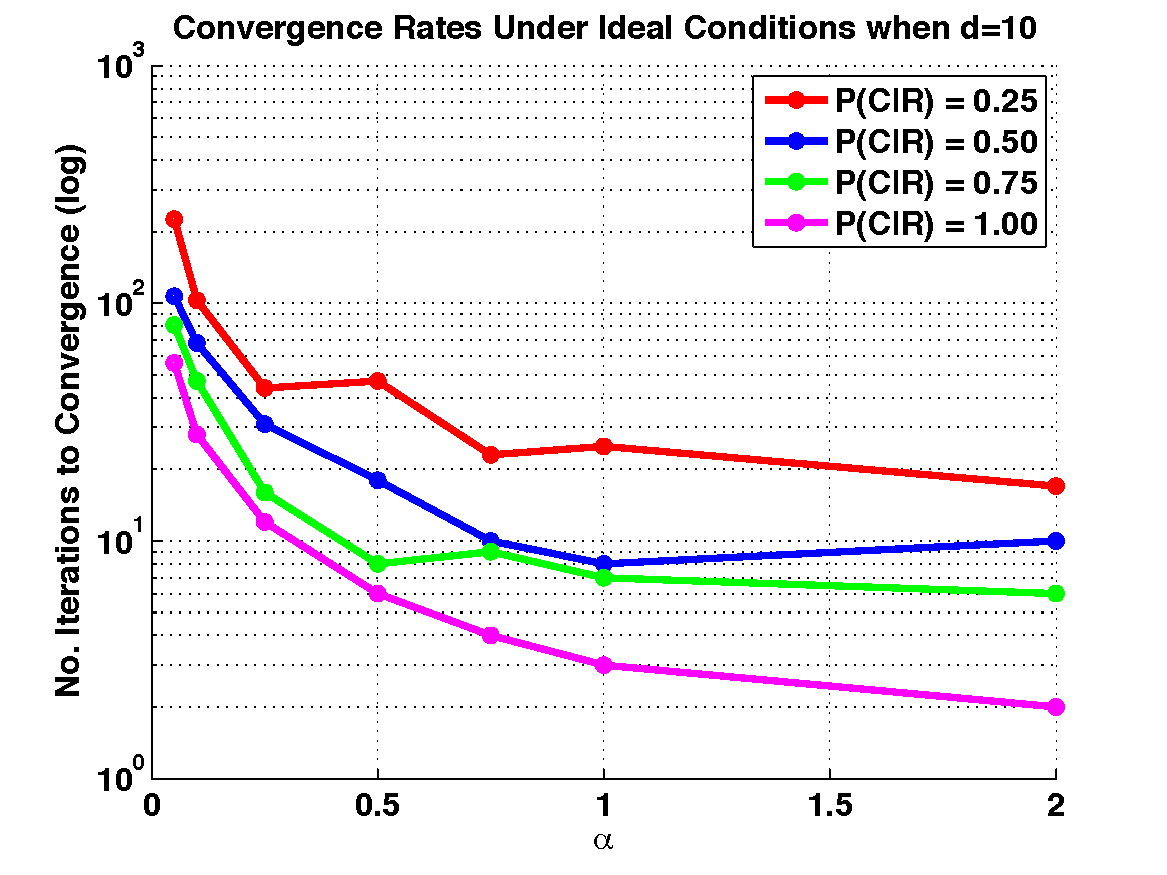
\includegraphics[width=\textwidth]{pics/perfect/simple_multiplicative_d10.pdf}
	  \caption{\textbf{Convergence @ $d=10$}}
	  \label{fig:sub1}
	\end{subfigure}%
	\begin{subfigure}{.33\textwidth}
	  \centering
	  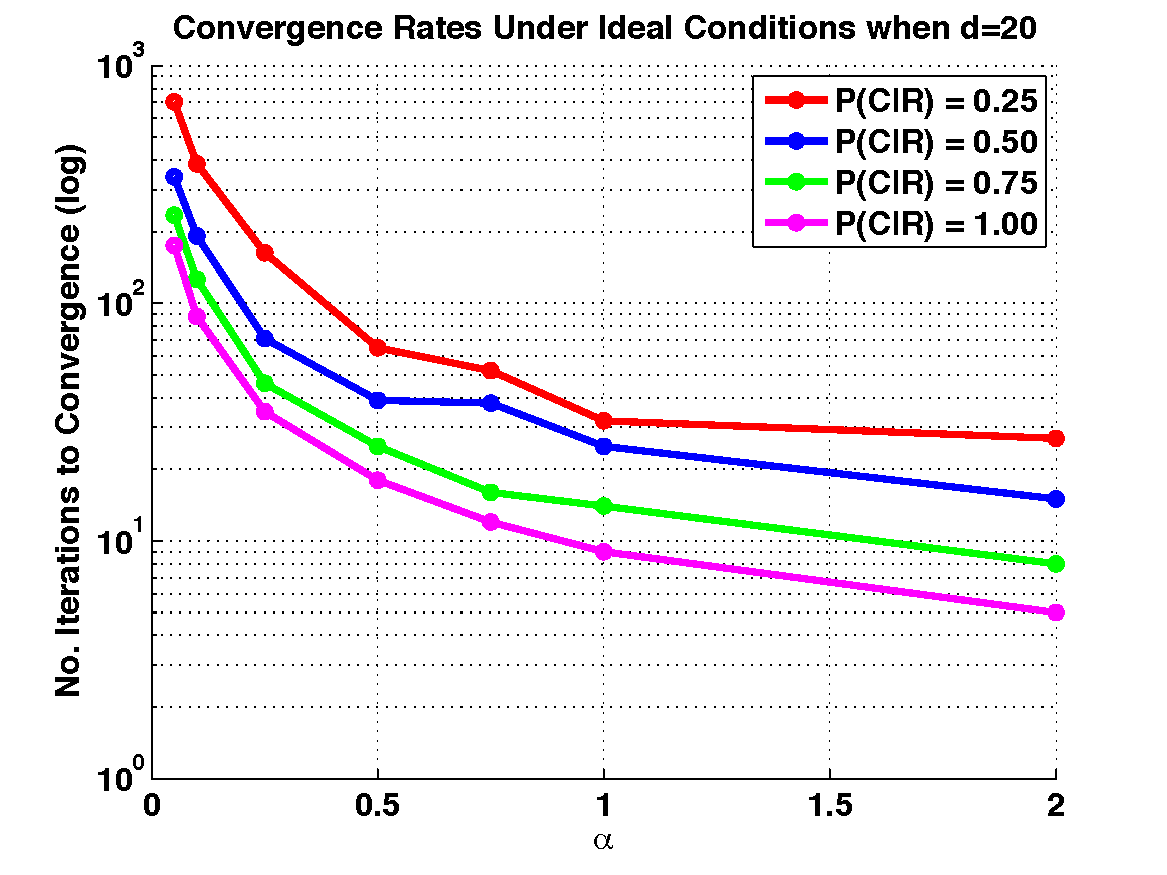
\includegraphics[width=\textwidth]{pics/perfect/simple_multiplicative_d20.pdf}
	  \caption{\textbf{Convergence @ $d=20$}}
	  \label{fig:sub2}
	\end{subfigure}
	\begin{subfigure}{.33\textwidth}
	  \centering
	  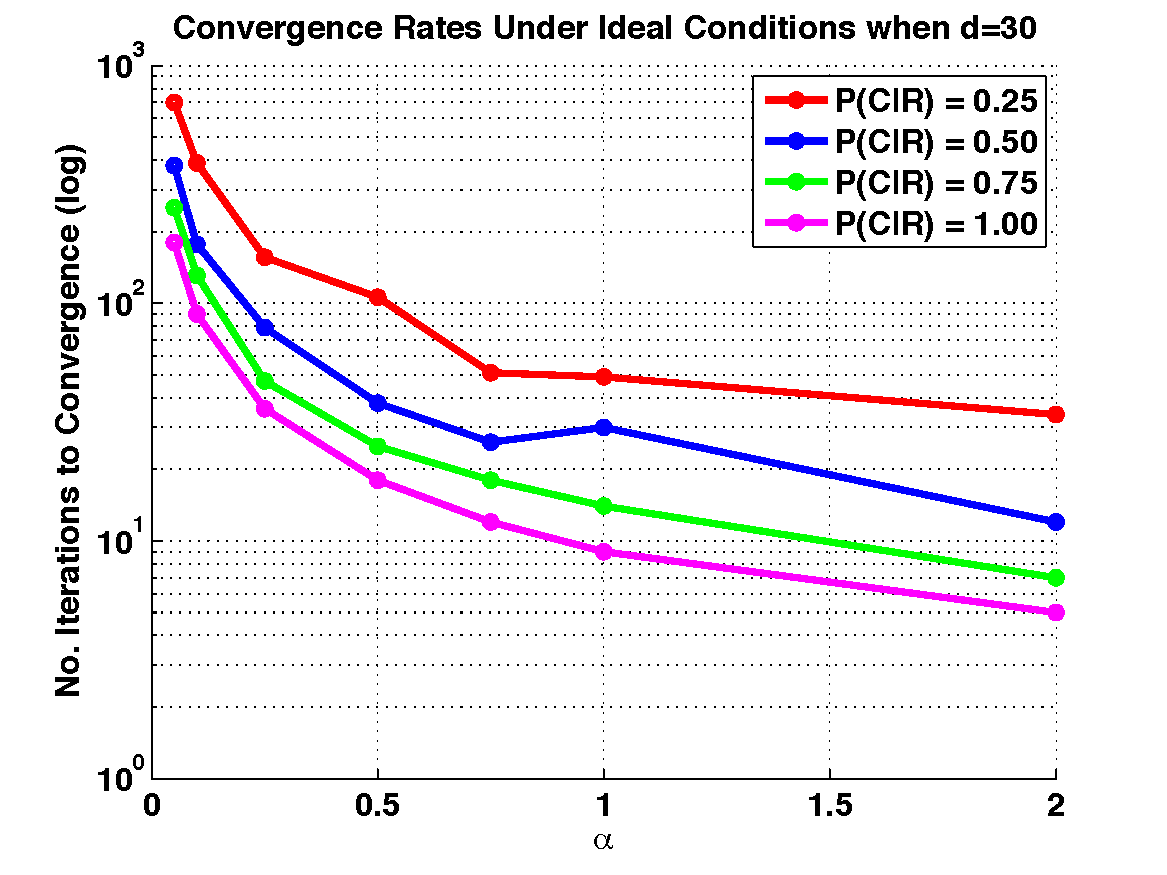
\includegraphics[width=\textwidth]{pics/perfect/simple_multiplicative_d30.pdf}
	  \caption{\textbf{Convergence @ $d=30$}}
	  \label{fig:sub2}
	\end{subfigure}
	
	\caption{\label{fig:perfect_convergence}\textbf{A series of graphs demonstrating the number of iterations required for performance to converge for given $\alpha$ values under ideal conditions. Each graph shows convergence times with varying depth levels.}}
\end{figure*}

Results for models \textbf{PD} and \textbf{PDE} are more complex. For variations of $P(C|R)$ when greater than 0.25, the two models exhibited an unusual behaviour. As the value for $P(C|R)$ was increased, we hypothesised that the number of iterations to reach maximum performance would reduce. Our results showed an almost consistent iteration count for each variation of $P(C|R)$ across the three values of 1.0, 0.75 and 0.5 - as can be seen in Tables \ref{tbl:results_perfect_demotive} and \ref{tbl:results_perfect_view} for models \textbf{PD} and \textbf{PDE} respectively.

\begin{figure}
	\begin{center}
	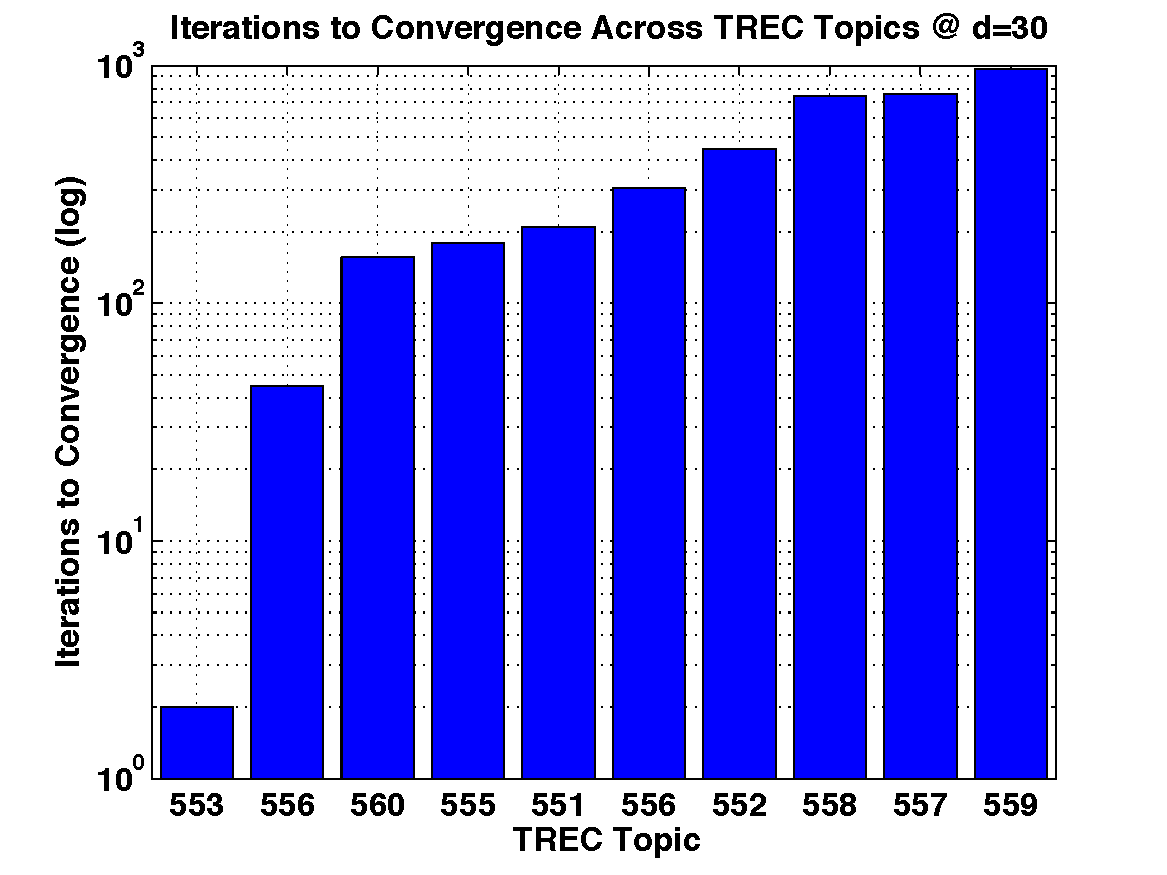
\includegraphics[width=\linewidth]{pics/perfect/perfect_different_topics.pdf}
	\end{center}
	\vspace{-0.5cm}
	\caption{\label{fig:perfect_different_topics}\textbf{A bar chart illustrating the different rates of convergence across TREC topics 551-560 for model \textbf{PD} with $P(C|R) = 0.25$ and $d=30$. Topics are ordered by the iteration count in ascending order.}\vspace{-0.4cm}}
\end{figure}

To examine this behaviour, we ran a further simulation running a sample of queries independently from one another. With model \textbf{PD} and a depth of 10 selected for TREC topics 551-650, we observed that for each query, a different number of iterations were required to reach maximum performance. Such behaviour would explain the consistent iteration count for varying levels of $P(C|R)$. While the performance of some queries may converge early - perhaps due to a potentially limited number of relevant documents high in their baseline rankings - they will almost certainly have to wait for slower queries - with a higher number of relevant documents - to reach maximum performance. With our simulations, as illustrated in Figure \ref{fig:perfect_different_topics}, many of these individual queries took a significant number of iterations to complete.

We also observed that a performance cliff exists for the demotion models, \textbf{PD} and \textbf{PDE}. With a low value of 0.25 set for $P(C|R)$, this meant that a relevant document had a 25\% chance of being clicked during each iteration. As can be seen in Tables \ref{tbl:results_perfect_demotive} and \ref{tbl:results_perfect_view}, such a small probability paired with a high $\beta$ value can have a significant negative impact, with the demotion aspect of each model dominating. Across all three depths for model \textbf{PD} when $P(C|R) = 0.25$ and $\beta = 2.0$, the maximum performance was achieved at the baseline - or 0\textsuperscript{th} iteration. This meant that all further iterations observed a drop in performance.

This finding provides a suggestion to a possible trade-off between the number of iterations that a site administrator would deem acceptable to notice a performance improvement, and the maximum performance he or she can obtain. Such a trade-off could perhaps be influenced by the number of visitors a given website receives, or how willing a particular site's audience would be to look further down results.

\subsection{Including Depth-Proportional Bias}
While clickthrough data are regarded as informative, it has been noted in several studies that such data are inherently biased by the trust they have in the results offered by the search engine used \cite{granka2004eyetracking, joachims2005clickthrough}. Positional bias reduces the probability of a document being examined the further down a ranked results list it appears. For example, a document at rank 1 would have a much higher chance of being examined than a document presented at rank 10.

To incorporate this issue in our study, we performed a series of simulations that examined performance when positional bias was added to clickthrough data. No longer perfect, the probability of examining (and potentially clicking) a document was then set to $1/r$ - or proportional to rank. Including such bias allowed us to address the following overarching question: \emph{what effects does positional bias have on retrieval performance?}

Our depth-proportional simulations were all run with a depth of 30 across all three models as our `perfect' simulations all offered their best performance at this depth. $d=30$ was also considered to be a relatively realistic depth that real-world users of search engines would be willing to look to. Like our `perfect world' simulations, we ran $P(C|R)$ with values of 1.0, 0.75, 0.5 and 0.25. The promotional tuning parameter $\alpha$ was set to a constant 0.75 throughout all simulations. Demotion tuning parameter $\beta$ was varied with the values 0.01, 0.05, 0.10, 0.25, 0.5, 0.75, 1.0 and 2.0 - we did however expect to see best performance from a low $\beta$ value based on our previous findings.

\subsubsection{Results}
To address the operational question posed above, we compared our findings against the results of our `perfect world' simulations. From a simplistic viewpoint, the performance obtained with our depth-proportional is broadly similar to our `perfect world' results. The key difference is however the time taken to reach that maximum performance. A larger number of iterations were required to achieve convergence, as the probability of viewing documents lower down rankings was less than 1.0.

\begin{figure}
	\begin{center}
	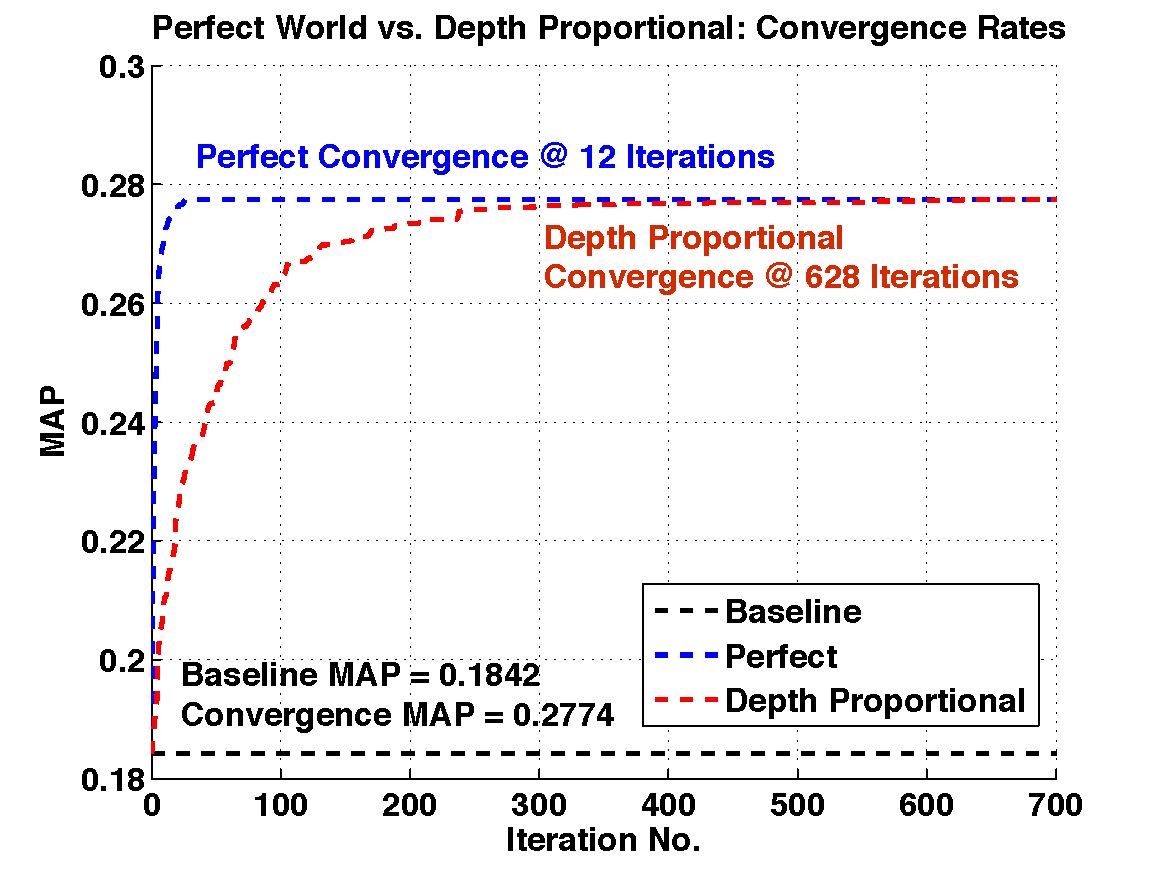
\includegraphics[width=\linewidth]{pics/bias/bias_iterations.pdf}
	\end{center}
	\vspace{-0.5cm}
	\caption{\label{fig:bias_iterations}\textbf{A line graph illustrating the difference in convergence rates for `perfect' and clickthrough data where the probability of viewing and clicking a document is proportional to a given document's depth. Data was generated by the \emph{P} model, where $\alpha = 0.75$, $P(C|R)=0.5$ and $d=30$ for each.}\vspace{-0.5cm}}
\end{figure}

This observation was noted from our promotion-only model \textbf{P}, which showed an identical maximum performance to ideal conditions. Moreover, the number of iterations required for convergence was influenced by the probability of clicking on a relevant document, $P(C|R)$. The higher $P(C|R)$, fewer iterations were required to reach convergence. The iteration count was still much higher than experienced under ideal conditions, as illustrated in Figure \ref{fig:bias_iterations} where ideal and depth-proportional results are compared with $P(C|R) = 0.5$. As the figure demonstrates, a comparable performance was achieved in little over 250 iterations, where MAP was evaluated to be 0.2757. This score was very close to the maximum attainable MAP of 0.2774.

\begin{table*}
	\renewcommand{\arraystretch}{1.3}
	\begin{center}
		\begin{small}
			\begin{tabularx}{\linewidth}{W{2.94cm}|W{1.4cm}|W{1.4cm}|W{1.4cm}|W{1.4cm}|W{1.4cm}|W{1.4cm}|W{1.4cm}|W{1.4cm}W{0.00000001cm}}
				
				& \centering{$\beta=0.01$}
				& \centering{$\beta=0.05$}
				& \centering{$\beta=0.1$}
				& \centering{$\beta=0.25$}
				& \centering{$\beta=0.5$}
				& \centering{$\beta=0.75$}
				& \centering{$\beta=1.0$}
				& \centering{$\beta=2.0$}&
				\tabularnewline[1em]
				\hline
				
				$P(C|R) = 0.0$
				& \multicolumn{8}{c}{\centering{{\tiny\textbf{PD}} 0.1842 ($i = 0$), {\tiny\textbf{PDE}} 0.1842 ($i = 0$)}}&
				\tabularnewline[1.4em]
				\hline
				\hline
				
				\multirow{2}{*}{\vspace{-0.45cm}$P(C|R) = 0.25$}
				& \centering{{\makebox[0pt][c]{{\tiny \textbf{PD}} \textbf{\emph{0.4374}}}\\\makebox[0pt][c]{{\tiny \textbf{PDE}} 0.2776}}}
				& \centering{{\makebox[0pt][c]{{\tiny \textbf{PD}} 0.3022}\\\makebox[0pt][c]{{\tiny \textbf{PDE}} 0.2848}}}
				& \centering{{\makebox[0pt][c]{{\tiny \textbf{PD}} 0.2173}\\\makebox[0pt][c]{{\tiny \textbf{PDE}} \textbf{\emph{0.2921}}}}}
				& \centering{{\makebox[0pt][c]{{\tiny \textbf{PD}} 0.1842}\\\makebox[0pt][c]{{\tiny \textbf{PDE}} 0.2858}}}
				& \centering{{\makebox[0pt][c]{{\tiny \textbf{PD}} 0.1842}\\\makebox[0pt][c]{{\tiny \textbf{PDE}} 0.2515}}}
				& \centering{{\makebox[0pt][c]{{\tiny \textbf{PD}} 0.1842}\\\makebox[0pt][c]{{\tiny \textbf{PDE}} 0.2335}}}
				& \centering{{\makebox[0pt][c]{{\tiny \textbf{PD}} 0.1842}\\\makebox[0pt][c]{{\tiny \textbf{PDE}} 0.2238}}}
				& \centering{{\makebox[0pt][c]{{\tiny \textbf{PD}} 0.1842}\\\makebox[0pt][c]{{\tiny \textbf{PDE}} 0.1842}}}&
				\tabularnewline[1.4em]
				\cline{2-9}
				
				& \centering{{\makebox[0pt][c]{{\tiny \textbf{PD}} $i=988$}\\\makebox[0pt][c]{{\tiny \textbf{PDE}} $i=924$}}}
				& \centering{{\makebox[0pt][c]{{\tiny \textbf{PD}} $i=513$}\\\makebox[0pt][c]{{\tiny \textbf{PDE}} $i=1000$}}}
				& \centering{{\makebox[0pt][c]{{\tiny \textbf{PD}} $i=88$}\\\makebox[0pt][c]{{\tiny \textbf{PDE}} $i=1000$}}}
				& \centering{{\makebox[0pt][c]{{\tiny \textbf{PD}} $i=0$}\\\makebox[0pt][c]{{\tiny \textbf{PDE}} $i=969$}}}
				& \centering{{\makebox[0pt][c]{{\tiny \textbf{PD}} $i=0$}\\\makebox[0pt][c]{{\tiny \textbf{PDE}} $i=890$}}}
				& \centering{{\makebox[0pt][c]{{\tiny \textbf{PD}} $i=0$}\\\makebox[0pt][c]{{\tiny \textbf{PDE}} $i=1000$}}}
				& \centering{{\makebox[0pt][c]{{\tiny \textbf{PD}} $i=0$}\\\makebox[0pt][c]{{\tiny \textbf{PDE}} $i=1000$}}}
				& \centering{{\makebox[0pt][c]{{\tiny \textbf{PD}} $i=0$}\\\makebox[0pt][c]{{\tiny \textbf{PDE}} $i=0$}}}&
				\tabularnewline[1.4em]
				\hline
				\hline
				
				\multirow{2}{*}{\vspace{-0.45cm}$P(C|R) = 0.5$}
				& \centering{{\makebox[0pt][c]{{\tiny \textbf{PD}} \textbf{\emph{0.4767}}}\\\makebox[0pt][c]{{\tiny \textbf{PDE}} 0.2776}}}
				& \centering{{\makebox[0pt][c]{{\tiny \textbf{PD}} 0.4263}\\\makebox[0pt][c]{{\tiny \textbf{PDE}} 0.2847}}}
				& \centering{{\makebox[0pt][c]{{\tiny \textbf{PD}} 0.3208}\\\makebox[0pt][c]{{\tiny \textbf{PDE}} 0.2881}}}
				& \centering{{\makebox[0pt][c]{{\tiny \textbf{PD}} 0.2139}\\\makebox[0pt][c]{{\tiny \textbf{PDE}} 0.3084}}}
				& \centering{{\makebox[0pt][c]{{\tiny \textbf{PD}} 0.1842}\\\makebox[0pt][c]{{\tiny \textbf{PDE}} \textbf{\emph{0.3226}}}}}
				& \centering{{\makebox[0pt][c]{{\tiny \textbf{PD}} 0.1842}\\\makebox[0pt][c]{{\tiny \textbf{PDE}} 0.3049}}}
				& \centering{{\makebox[0pt][c]{{\tiny \textbf{PD}} 0.1842}\\\makebox[0pt][c]{{\tiny \textbf{PDE}} 0.2614}}}
				& \centering{{\makebox[0pt][c]{{\tiny \textbf{PD}} 0.1842}\\\makebox[0pt][c]{{\tiny \textbf{PDE}} 0.2618}}}&
				\tabularnewline[1.4em]
				\cline{2-9}
				
				& \centering{{\makebox[0pt][c]{{\tiny \textbf{PD}} $i=1000$}\\\makebox[0pt][c]{{\tiny \textbf{PDE}} $i=501$}}}
				& \centering{{\makebox[0pt][c]{{\tiny \textbf{PD}} $i=1000$}\\\makebox[0pt][c]{{\tiny \textbf{PDE}} $i=812$}}}
				& \centering{{\makebox[0pt][c]{{\tiny \textbf{PD}} $i=211$}\\\makebox[0pt][c]{{\tiny \textbf{PDE}} $i=1000$}}}
				& \centering{{\makebox[0pt][c]{{\tiny \textbf{PD}} $i=23$}\\\makebox[0pt][c]{{\tiny \textbf{PDE}} $i=1000$}}}
				& \centering{{\makebox[0pt][c]{{\tiny \textbf{PD}} $i=0$}\\\makebox[0pt][c]{{\tiny \textbf{PDE}} $i=1000$}}}
				& \centering{{\makebox[0pt][c]{{\tiny \textbf{PD}} $i=0$}\\\makebox[0pt][c]{{\tiny \textbf{PDE}} $i=1000$}}}
				& \centering{{\makebox[0pt][c]{{\tiny \textbf{PD}} $i=0$}\\\makebox[0pt][c]{{\tiny \textbf{PDE}} $i=305$}}}
				& \centering{{\makebox[0pt][c]{{\tiny \textbf{PD}} $i=0$}\\\makebox[0pt][c]{{\tiny \textbf{PDE}} $i=977$}}}&
				\tabularnewline[1.4em]
				\hline
				\hline
				
				\multirow{2}{*}{\vspace{-0.45cm}$P(C|R) = 0.75$}
				& \centering{{\makebox[0pt][c]{{\tiny \textbf{PD}} 0.4938}\\\makebox[0pt][c]{{\tiny \textbf{PDE}} 0.2776}}}
				& \centering{{\makebox[0pt][c]{{\tiny \textbf{PD}} \textbf{\emph{0.4985}}}\\\makebox[0pt][c]{{\tiny \textbf{PDE}} 0.281}}}
				& \centering{{\makebox[0pt][c]{{\tiny \textbf{PD}} 0.3852}\\\makebox[0pt][c]{{\tiny \textbf{PDE}} 0.2884}}}
				& \centering{{\makebox[0pt][c]{{\tiny \textbf{PD}} 0.2569}\\\makebox[0pt][c]{{\tiny \textbf{PDE}} 0.3076}}}
				& \centering{{\makebox[0pt][c]{{\tiny \textbf{PD}} 0.2072}\\\makebox[0pt][c]{{\tiny \textbf{PDE}} 0.3257}}}
				& \centering{{\makebox[0pt][c]{{\tiny \textbf{PD}} 0.1939}\\\makebox[0pt][c]{{\tiny \textbf{PDE}} 0.3323}}}
				& \centering{{\makebox[0pt][c]{{\tiny \textbf{PD}} 0.1842}\\\makebox[0pt][c]{{\tiny \textbf{PDE}} 0.3355}}}
				& \centering{{\makebox[0pt][c]{{\tiny \textbf{PD}} 0.1842}\\\makebox[0pt][c]{{\tiny \textbf{PDE}} \emph{\textbf{0.3377}}}}}&
				\tabularnewline[1.4em]
				\cline{2-9}
				
				& \centering{{\makebox[0pt][c]{{\tiny \textbf{PD}} $i=1000$}\\\makebox[0pt][c]{{\tiny \textbf{PDE}} $i=350$}}}
				& \centering{{\makebox[0pt][c]{{\tiny \textbf{PD}} $i=981$}\\\makebox[0pt][c]{{\tiny \textbf{PDE}} $i=314$}}}
				& \centering{{\makebox[0pt][c]{{\tiny \textbf{PD}} $i=413$}\\\makebox[0pt][c]{{\tiny \textbf{PDE}} $i=951$}}}
				& \centering{{\makebox[0pt][c]{{\tiny \textbf{PD}} $i=143$}\\\makebox[0pt][c]{{\tiny \textbf{PDE}} $i=974$}}}
				& \centering{{\makebox[0pt][c]{{\tiny \textbf{PD}} $i=18$}\\\makebox[0pt][c]{{\tiny \textbf{PDE}} $i=1000$}}}
				& \centering{{\makebox[0pt][c]{{\tiny \textbf{PD}} $i=8$}\\\makebox[0pt][c]{{\tiny \textbf{PDE}} $i=1000$}}}
				& \centering{{\makebox[0pt][c]{{\tiny \textbf{PD}} $i=0$}\\\makebox[0pt][c]{{\tiny \textbf{PDE}} $i=1000$}}}
				& \centering{{\makebox[0pt][c]{{\tiny \textbf{PD}} $i=0$}\\\makebox[0pt][c]{{\tiny \textbf{PDE}} $i=1000$}}}&
				\tabularnewline[1.4em]
				\hline
				\hline
				
				\multirow{2}{*}{\vspace{-0.45cm}$P(C|R) = 1.0$}
				& \centering{{\makebox[0pt][c]{{\tiny \textbf{PD}} 0.4998}\\\makebox[0pt][c]{{\tiny \textbf{PDE}} 0.2774}}}
				& \centering{{\makebox[0pt][c]{{\tiny \textbf{PD}} \textbf{0.5417}}\\\makebox[0pt][c]{{\tiny \textbf{PDE}} 0.2847}}}
				& \centering{{\makebox[0pt][c]{{\tiny \textbf{PD}} 0.4464}\\\makebox[0pt][c]{{\tiny \textbf{PDE}} 0.2894}}}
				& \centering{{\makebox[0pt][c]{{\tiny \textbf{PD}} 0.2868}\\\makebox[0pt][c]{{\tiny \textbf{PDE}} 0.3088}}}
				& \centering{{\makebox[0pt][c]{{\tiny \textbf{PD}} 0.2169}\\\makebox[0pt][c]{{\tiny \textbf{PDE}} 0.3261}}}
				& \centering{{\makebox[0pt][c]{{\tiny \textbf{PD}} 0.2171}\\\makebox[0pt][c]{{\tiny \textbf{PDE}} 0.3319}}}
				& \centering{{\makebox[0pt][c]{{\tiny \textbf{PD}} 0.1842}\\\makebox[0pt][c]{{\tiny \textbf{PDE}} 0.3379}}}
				& \centering{{\makebox[0pt][c]{{\tiny \textbf{PD}} 0.1842}\\\makebox[0pt][c]{{\tiny \textbf{PDE}} \textbf{0.3489}}}}&
				\tabularnewline[1.4em]
				\cline{2-9}
				
				& \centering{{\makebox[0pt][c]{{\tiny \textbf{PD}} $i=1000$}\\\makebox[0pt][c]{{\tiny \textbf{PDE}} $i=277$}}}
				& \centering{{\makebox[0pt][c]{{\tiny \textbf{PD}} $i=978$}\\\makebox[0pt][c]{{\tiny \textbf{PDE}} $i=819$}}}
				& \centering{{\makebox[0pt][c]{{\tiny \textbf{PD}} $i=979$}\\\makebox[0pt][c]{{\tiny \textbf{PDE}} $i=1000$}}}
				& \centering{{\makebox[0pt][c]{{\tiny \textbf{PD}} $i=173$}\\\makebox[0pt][c]{{\tiny \textbf{PDE}} $i=1000$}}}
				& \centering{{\makebox[0pt][c]{{\tiny \textbf{PD}} $i=27$}\\\makebox[0pt][c]{{\tiny \textbf{PDE}} $i=1000$}}}
				& \centering{{\makebox[0pt][c]{{\tiny \textbf{PD}} $i=16$}\\\makebox[0pt][c]{{\tiny \textbf{PDE}} $i=1000$}}}
				& \centering{{\makebox[0pt][c]{{\tiny \textbf{PD}} $i=0$}\\\makebox[0pt][c]{{\tiny \textbf{PDE}} $i=1000$}}}
				& \centering{{\makebox[0pt][c]{{\tiny \textbf{PD}} $i=0$}\\\makebox[0pt][c]{{\tiny \textbf{PDE}} $i=1000$}}}&
				\tabularnewline[1.4em]
				
			\end{tabularx}
		\end{small}
	\end{center}

	\vspace{-0.4cm}
	\caption{\textbf{Table highlighting the best MAP values obtained and corresponding simulation counts for models \emph{PD} and \emph{PDE} with depth-proportional clickthrough data. $P(C|R)$ is varied, and both $d=30$ and $\alpha=0.75$ are constant.}}
	\label{tbl:results_biased_demotion}
\end{table*}

Despite these intuitive findings, interesting observations were made with the two promotion/demotion models, \textbf{PD} and \textbf{PDE}. For \textbf{PD}, it was observed that performance was at its highest when $\beta$ was set to a low value. When $P(C|R)$ was also set to a low value of 0.25, a MAP of 0.4374 was obtained when $\beta = 0.01$. This value is higher than the MAP of 0.3022 observed for $\beta = 0.05$. However, with $P(C|R)$ set to 1.0, the best performance of 0.5417 was attained with $\beta = 0.05$.

This finding suggests that there is a possible relationship between the probability of clicks on a relevant document, $P(C|R)$, and the weighting applied to the demotion aspect of clickthrough models, $\beta$. If for example users of a website search engine were to click on more and more relevant documents, the demotion weighting can be \emph{slightly} increased due to the increased confidence in users' clicks signifying relevance to a query. The greater weighting for demotion would therefore allow documents that are considered irrelevant to be demoted down rankings more quickly, yielding a greater performance gain. Care must be taken regarding the choice of $\beta$ value - as seen in Table \ref{tbl:results_biased_demotion}, a $\beta$ value greater than 0.05 gave steadily reduced performance - dropping below baseline values for high $\beta$ values.

Also shown in Table \ref{tbl:results_biased_demotion} are our results for \textbf{PDE}. Compared to \textbf{PD}, we found significant differences in the way the model reacted to differing parameter variations. As expected, better performance was observed as $P(C|R)$ increased. However, as $\beta$ increased, so did performance - even past the \textbf{PD} threshold of 0.05. Indeed, the highest MAP of 0.3489 for \textbf{PDE} was observed when $P(C|R) = 1.0$ and $\beta = 2.0$. Such behaviour could be attributed to the greater demoting power \textbf{PDE} had as $\beta$ increased. Examining the definition of the model in Equation \ref{eqn:pde}, the greater the chance the demotion aspect of the model would dominate the promotion aspect as $\beta$ was set to a higher value. Increasing $\beta$ therefore attempted to mitigate the effect of introducing depth-proportional bias.

\subsection{Varying Noise}
One of the major disadvantages of clickthrough data are its tendency of being susceptible to noise. Noise - where users click on documents that are irrelevant to a query - cannot be avoided in a real-world environment. Thus, any models developed that utilise clickthrough data must have a degree of tolerance to noise - which inevitably comes with the sacrifice of performance. This therefore leads us to ask the operational question: \emph{how does including noise in clickthrough data affect performance?}

To address this question, we conducted a further series of simulations. Coupled with positional bias, we began to vary the probability of a click on irrelevant documents, $P(C|N)$, along with $P(C|R)$. Up until this point, all simulations had been run free of noise, with $P(C|N) = 0.0$. With these simulations, we also set the probability of examining a document to be proportional to depth, and like previous simulations, set $\alpha = 0.75$. For our promotion/demotion models, $\beta$ was fixed at 0.05 due to the positive outcomes the value had with previous simulations. However, findings of our depth-proportional simulations pushed us towards running further simulations for models \textbf{PD} and \textbf{PDE} where $\beta$ was set to 0.10, 0.25 and 2.0. These simulations were then repeated without positional bias, allowing us to make a direct comparison with our `perfect world' simulations.

\subsubsection{Results}\label{sec:results:noise}
Results from our simulations incorporating noise show that performance is affected - in terms of the maximum that can be attained, and the length of time required to reach it. Previous simulations have demonstrated that the behaviour of model \textbf{P} has been straightforward to follow. We therefore use the results from \textbf{P} to explain basic behavioural changes with clickthrough data as noise is varied.

Table \ref{tbl:noisy_multiplicative} shows the highest MAP figures obtained for varying levels of $P(C|R)$ and $P(C|N)$ across clickthrough simulations incorporating noise, and noise with depth-proportional viewing. The table also shows the number of iterations that were required to reach the performance highs.

\begin{figure}[t!]
	\begin{center}
	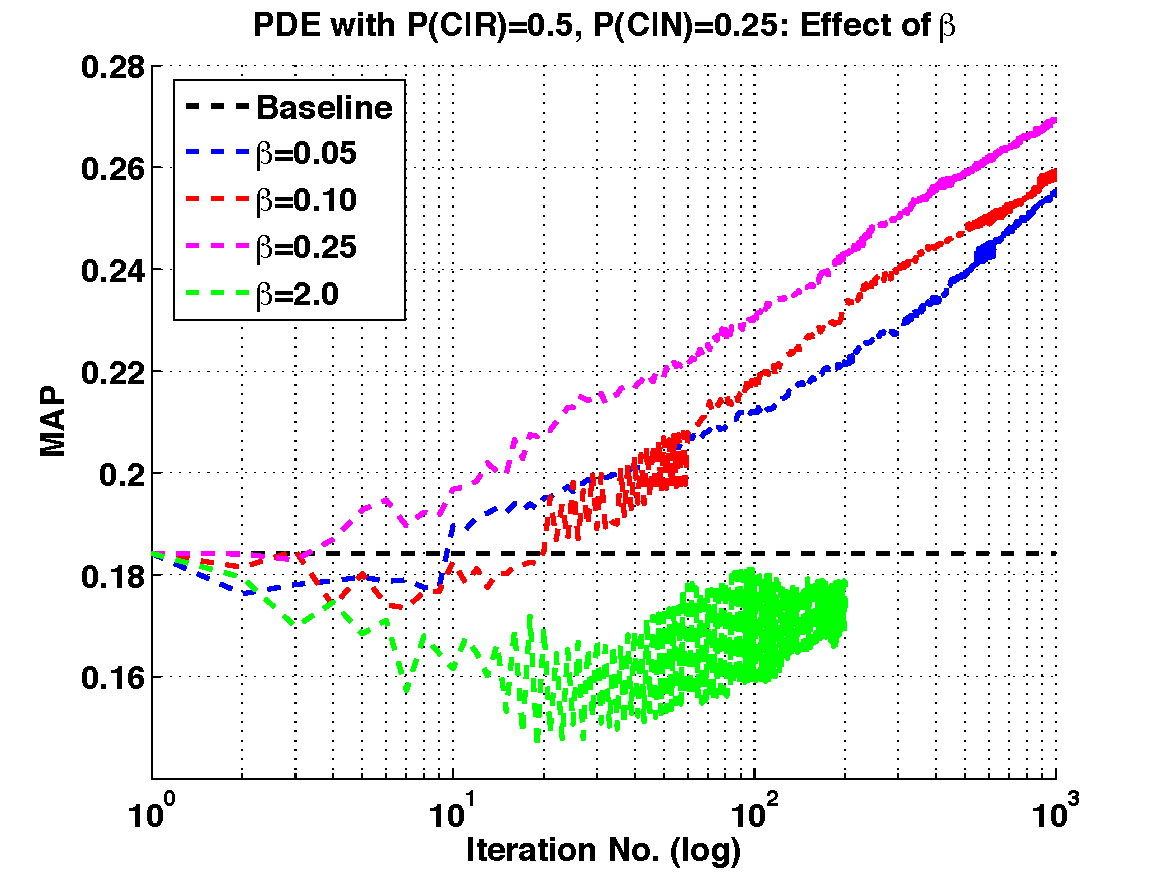
\includegraphics[width=\linewidth]{pics/noise/noise_pde_beta.pdf}
	\end{center}
	\vspace{-0.5cm}
	\caption{\label{fig:noise_pde_beta}\textbf{A line graph illustrating performance vs. iterations with different $\beta$ values for \emph{PDE} using noisy data and depth-proportional views. Here, $P(C|R) = 0.5$ and $P(C|N) = 0.25$.}\vspace{-0.25cm}}
\end{figure}

Our results show that as $P(C|R)$ increases, performance also increases. However, as we begin to introduce noise by increasing the value of $P(C|N)$, we observe two key behaviours which are exerted:

\begin{enumerate}
	
	\item{convergence to maximum performance takes significantly longer; or}
	
	\item{no performance improvement is observed whatsoever.}
	
\end{enumerate}

To provide an example of the former observation, we can see from Table \ref{tbl:noisy_multiplicative} that when $P(C|R) = 0.5$ and $P(C|N) = 0.25$, performance for our noise-only simulation converged at the highest attainable MAP of 0.2774 after 82 iterations. This is in comparison to the 12 iterations that our simulations run ideal conditions took (see Table \ref{tbl:results_perfect_demotive}). We also observed that including positional bias in our simulations increases the number of iterations required for convergence to 992 (with a cap at 1000) - and would require even more to reach the maximum attainable MAP of 0.2774.

Results also show a significant drop in performance as noise is introduced. This can be partly explained by the na\"{i}vety of \textbf{P}, detailed in Section \ref{sec:method:models:promo}. As $P(C|N)$ is increased, more irrelevant documents are clicked and promoted. As \textbf{P} assumes clicks signify relevance, tolerances for noise with the model are therefore low.

\begin{table}[t!]
	\renewcommand{\arraystretch}{1.3}
	\begin{center}
		\begin{small}
			\begin{tabularx}{\linewidth}{W{1.29cm}|W{1.29cm}|W{1.29cm}|W{1.29cm}|W{1.29cm}W{0.00000001cm}}
				
			 	& \centering{{\makebox[0pt][c]{$PN = 0.25$}}} & \centering{$PN = 0.5$} & \centering{{\makebox[0pt][c]{$PN = 0.75$}}} & \centering{$PN = 1.0$}&
				\tabularnewline[1.4em]
				\hline
				
				\multirow{2}{*}{\vspace{-0.45cm}$PR = 0.25$}
				& \centering{{\makebox[0pt][c]{{\tiny \textbf{ND}} 0.1842}\\\makebox[0pt][c]{{\tiny \textbf{N}} 0.1842}}}
				& \centering{{\makebox[0pt][c]{{\tiny \textbf{ND}} 0.1842}\\\makebox[0pt][c]{{\tiny \textbf{N}} 0.1842}}}
				& \centering{{\makebox[0pt][c]{{\tiny \textbf{ND}} 0.1842}\\\makebox[0pt][c]{{\tiny \textbf{N}} 0.1842}}}
				& \centering{{\makebox[0pt][c]{{\tiny \textbf{ND}} 0.1842}\\\makebox[0pt][c]{{\tiny \textbf{N}} 0.1842}}}&
				\tabularnewline[1.4em]
				\cline{2-5}
				
				& \centering{{\makebox[0pt][c]{{\tiny \textbf{ND}} $i=0$}\\\makebox[0pt][c]{{\tiny \textbf{N}} $i=0$}}}
				& \centering{{\makebox[0pt][c]{{\tiny \textbf{ND}} $i=0$}\\\makebox[0pt][c]{{\tiny \textbf{N}} $i=0$}}}
				& \centering{{\makebox[0pt][c]{{\tiny \textbf{ND}} $i=0$}\\\makebox[0pt][c]{{\tiny \textbf{N}} $i=0$}}}
				& \centering{{\makebox[0pt][c]{{\tiny \textbf{ND}} $i=0$}\\\makebox[0pt][c]{{\tiny \textbf{N}} $i=0$}}}&
				\tabularnewline[1.4em]
				\hline
				
				\multirow{2}{*}{\vspace{-0.45cm}$PR = 0.5$}
				& \centering{{\makebox[0pt][c]{{\tiny \textbf{ND}} \textbf{0.2527}}\\\makebox[0pt][c]{{\tiny \textbf{N}} \textbf{0.2774}}}}
				& \centering{{\makebox[0pt][c]{{\tiny \textbf{ND}} 0.1842}\\\makebox[0pt][c]{{\tiny \textbf{N}} 0.1842}}}
				& \centering{{\makebox[0pt][c]{{\tiny \textbf{ND}} 0.1842}\\\makebox[0pt][c]{{\tiny \textbf{N}} 0.1842}}}
				& \centering{{\makebox[0pt][c]{{\tiny \textbf{ND}} 0.1842}\\\makebox[0pt][c]{{\tiny \textbf{N}} 0.1842}}}&
				\tabularnewline[1.4em]
				\cline{2-5}
				
				& \centering{{\makebox[0pt][c]{{\tiny \textbf{ND}} $i=992$}\\\makebox[0pt][c]{{\tiny \textbf{N}} $i=82$}}}
				& \centering{{\makebox[0pt][c]{{\tiny \textbf{ND}} $i=0$}\\\makebox[0pt][c]{{\tiny \textbf{N}} $i=0$}}}
				& \centering{{\makebox[0pt][c]{{\tiny \textbf{ND}} $i=0$}\\\makebox[0pt][c]{{\tiny \textbf{N}} $i=0$}}}
				& \centering{{\makebox[0pt][c]{{\tiny \textbf{ND}} $i=0$}\\\makebox[0pt][c]{{\tiny \textbf{N}} $i=0$}}}&
				\tabularnewline[1.4em]
				\hline
				
				\multirow{2}{*}{\vspace{-0.45cm}$PR = 0.75$}
				& \centering{{\makebox[0pt][c]{{\tiny \textbf{ND}} \textbf{0.2769}}\\\makebox[0pt][c]{{\tiny \textbf{N}} \textbf{0.2774}}}}
				& \centering{{\makebox[0pt][c]{{\tiny \textbf{ND}} \textbf{0.2291}}\\\makebox[0pt][c]{{\tiny \textbf{N}} \textbf{0.2774}}}}
				& \centering{{\makebox[0pt][c]{{\tiny \textbf{ND}} \textbf{0.1884}}\\\makebox[0pt][c]{{\tiny \textbf{N}} 0.1842}}}
				& \centering{{\makebox[0pt][c]{{\tiny \textbf{ND}} 0.1842}\\\makebox[0pt][c]{{\tiny \textbf{N}} 0.1842}}}&
				\tabularnewline[1.4em]
				\cline{2-5}
				
				& \centering{{\makebox[0pt][c]{{\tiny \textbf{ND}} $i=947$}\\\makebox[0pt][c]{{\tiny \textbf{N}} $i=39$}}}
				& \centering{{\makebox[0pt][c]{{\tiny \textbf{ND}} $i=997$}\\\makebox[0pt][c]{{\tiny \textbf{N}} $i=95$}}}
				& \centering{{\makebox[0pt][c]{{\tiny \textbf{ND}} $i=1$}\\\makebox[0pt][c]{{\tiny \textbf{N}} $i=0$}}}
				& \centering{{\makebox[0pt][c]{{\tiny \textbf{ND}} $i=0$}\\\makebox[0pt][c]{{\tiny \textbf{N}} $i=0$}}}&
				\tabularnewline[1.4em]
				\hline
				
				\multirow{2}{*}{\vspace{-0.45cm}$PR = 1.0$}
				& \centering{{\makebox[0pt][c]{{\tiny \textbf{ND}} \textbf{0.2774}}\\\makebox[0pt][c]{{\tiny \textbf{N}} \textbf{0.2774}}}}
				& \centering{{\makebox[0pt][c]{{\tiny \textbf{ND}} \textbf{0.2625}}\\\makebox[0pt][c]{{\tiny \textbf{N}} \textbf{0.2774}}}}
				& \centering{{\makebox[0pt][c]{{\tiny \textbf{ND}} \textbf{0.2176}}\\\makebox[0pt][c]{{\tiny \textbf{N}} \textbf{0.2774}}}}
				& \centering{{\makebox[0pt][c]{{\tiny \textbf{ND}} \textbf{0.1845}}\\\makebox[0pt][c]{{\tiny \textbf{N}} 0.1842}}}&
				\tabularnewline[1.4em]
				\cline{2-5}
				
				& \centering{{\makebox[0pt][c]{{\tiny \textbf{ND}} $i=713$}\\\makebox[0pt][c]{{\tiny \textbf{N}} $i=16$}}}
				& \centering{{\makebox[0pt][c]{{\tiny \textbf{ND}} $i=999$}\\\makebox[0pt][c]{{\tiny \textbf{N}} $i=29$}}}
				& \centering{{\makebox[0pt][c]{{\tiny \textbf{ND}} $i=983$}\\\makebox[0pt][c]{{\tiny \textbf{N}} $i=66$}}}
				& \centering{{\makebox[0pt][c]{{\tiny \textbf{ND}} $i=2$}\\\makebox[0pt][c]{{\tiny \textbf{N}} $i=0$}}}&
				\tabularnewline[1.4em]
				
			\end{tabularx}
		\end{small}
	\end{center}
	
	\vspace{-0.4cm}
	\caption{\textbf{Table illustrating the highest MAP values obtained and associated iteration counts for model \emph{P}, with variations in the probabilities for relevant and irrelevant clicks. Data in the table is for noise and depth-proportional \emph{(ND)}, and noise only \emph{(N)}. For brevity, \emph{PR} in this table signifies $P(C|R)$, and \emph{PN} signifies $P(C|N)$. The baseline MAP was 0.1842, and the maximum attainable MAP at $d=30$ was 0.2774.}\vspace{-0.4cm}}
	\label{tbl:noisy_multiplicative}
\end{table}

Results from our promotion/demotion models \textbf{PD} and \textbf{PDE} followed a similar trend to those of \textbf{P}. Although a similar performance `cliff' existed whereafter no improvements were made, we did observe notable increases over \textbf{P} before the `cliff' was reached. Performance also dropped at a much slower rate, suggesting that \textbf{PD} and \textbf{PDE} were much more tolerable to noise. Tables \hyperref[tbl:noisy_pd]{7} and \hyperref[tbl:noisy_pde]{8} present the highest attained MAP values and respective iteration counts for models \textbf{PD} and \textbf{PDE} respectively.

\begin{table*}

	\begin{subtable}{\columnwidth}
			\begin{small}
				\begin{tabularx}{\linewidth}{W{1.29cm}|W{1.29cm}|W{1.29cm}|W{1.29cm}|W{1.29cm}W{0.00000001cm}}

				 	\centering{{\makebox[0pt][c]{{\tiny \textbf{ND}} $\beta = 0.05$}\\\makebox[0pt][c]{{\tiny \textbf{N}} $\beta = 2.0$}}}
					& \centering{{\makebox[0pt][c]{$PN = 0.25$}}} & \centering{$PN = 0.5$} & \centering{{\makebox[0pt][c]{$PN = 0.75$}}} & \centering{$PN = 1.0$}&
					\tabularnewline[1.4em]
					\hline

					\multirow{2}{*}{\vspace{-0.45cm}$PR = 0.25$}
					& \centering{{\makebox[0pt][c]{{\tiny \textbf{ND}} 0.1842}\\\makebox[0pt][c]{{\tiny \textbf{N}} 0.1842}}}
					& \centering{{\makebox[0pt][c]{{\tiny \textbf{ND}} 0.1842}\\\makebox[0pt][c]{{\tiny \textbf{N}} 0.1842}}}
					& \centering{{\makebox[0pt][c]{{\tiny \textbf{ND}} 0.1842}\\\makebox[0pt][c]{{\tiny \textbf{N}} 0.1842}}}
					& \centering{{\makebox[0pt][c]{{\tiny \textbf{ND}} 0.1842}\\\makebox[0pt][c]{{\tiny \textbf{N}} 0.1842}}}&
					\tabularnewline[1.4em]
					\cline{2-5}

					& \centering{{\makebox[0pt][c]{{\tiny \textbf{ND}} $i=0$}\\\makebox[0pt][c]{{\tiny \textbf{N}} $i=0$}}}
					& \centering{{\makebox[0pt][c]{{\tiny \textbf{ND}} $i=0$}\\\makebox[0pt][c]{{\tiny \textbf{N}} $i=0$}}}
					& \centering{{\makebox[0pt][c]{{\tiny \textbf{ND}} $i=0$}\\\makebox[0pt][c]{{\tiny \textbf{N}} $i=0$}}}
					& \centering{{\makebox[0pt][c]{{\tiny \textbf{ND}} $i=0$}\\\makebox[0pt][c]{{\tiny \textbf{N}} $i=0$}}}&
					\tabularnewline[1.4em]
					\hline

					\multirow{2}{*}{\vspace{-0.45cm}$PR = 0.5$}
					& \centering{{\makebox[0pt][c]{{\tiny \textbf{ND}} \textbf{0.2350}}\\\makebox[0pt][c]{{\tiny \textbf{N}} 0.1842}}}
					& \centering{{\makebox[0pt][c]{{\tiny \textbf{ND}} 0.1842}\\\makebox[0pt][c]{{\tiny \textbf{N}} 0.1842}}}
					& \centering{{\makebox[0pt][c]{{\tiny \textbf{ND}} 0.1842}\\\makebox[0pt][c]{{\tiny \textbf{N}} 0.1842}}}
					& \centering{{\makebox[0pt][c]{{\tiny \textbf{ND}} 0.1842}\\\makebox[0pt][c]{{\tiny \textbf{N}} 0.1842}}}&
					\tabularnewline[1.4em]
					\cline{2-5}

					& \centering{{\makebox[0pt][c]{{\tiny \textbf{ND}} $i=416$}\\\makebox[0pt][c]{{\tiny \textbf{N}} $i=0$}}}
					& \centering{{\makebox[0pt][c]{{\tiny \textbf{ND}} $i=0$}\\\makebox[0pt][c]{{\tiny \textbf{N}} $i=0$}}}
					& \centering{{\makebox[0pt][c]{{\tiny \textbf{ND}} $i=0$}\\\makebox[0pt][c]{{\tiny \textbf{N}} $i=0$}}}
					& \centering{{\makebox[0pt][c]{{\tiny \textbf{ND}} $i=0$}\\\makebox[0pt][c]{{\tiny \textbf{N}} $i=0$}}}&
					\tabularnewline[1.4em]
					\hline

					\multirow{2}{*}{\vspace{-0.45cm}$PR = 0.75$}
					& \centering{{\makebox[0pt][c]{{\tiny \textbf{ND}} \textbf{0.4000}}\\\makebox[0pt][c]{{\tiny \textbf{N}} \textbf{0.6132}}}}
					& \centering{{\makebox[0pt][c]{{\tiny \textbf{ND}} \textbf{0.2102}}\\\makebox[0pt][c]{{\tiny \textbf{N}} \textbf{0.5472}}}}
					& \centering{{\makebox[0pt][c]{{\tiny \textbf{ND}} 0.1842}\\\makebox[0pt][c]{{\tiny \textbf{N}} 0.1842}}}
					& \centering{{\makebox[0pt][c]{{\tiny \textbf{ND}} 0.1842}\\\makebox[0pt][c]{{\tiny \textbf{N}} 0.1842}}}&
					\tabularnewline[1.4em]
					\cline{2-5}

					& \centering{{\makebox[0pt][c]{{\tiny \textbf{ND}} $i=978$}\\\makebox[0pt][c]{{\tiny \textbf{N}} $i=915$}}}
					& \centering{{\makebox[0pt][c]{{\tiny \textbf{ND}} $i=760$}\\\makebox[0pt][c]{{\tiny \textbf{N}} $i=984$}}}
					& \centering{{\makebox[0pt][c]{{\tiny \textbf{ND}} $i=0$}\\\makebox[0pt][c]{{\tiny \textbf{N}} $i=0$}}}
					& \centering{{\makebox[0pt][c]{{\tiny \textbf{ND}} $i=0$}\\\makebox[0pt][c]{{\tiny \textbf{N}} $i=0$}}}&
					\tabularnewline[1.4em]
					\hline

					\multirow{2}{*}{\vspace{-0.45cm}$PR = 1.0$}
					& \centering{{\makebox[0pt][c]{{\tiny \textbf{ND}} \textbf{0.467}}\\\makebox[0pt][c]{{\tiny \textbf{N}} \textbf{0.6724}}}}
					& \centering{{\makebox[0pt][c]{{\tiny \textbf{ND}} \textbf{0.3241}}\\\makebox[0pt][c]{{\tiny \textbf{N}} \textbf{0.6719}}}}
					& \centering{{\makebox[0pt][c]{{\tiny \textbf{ND}} \textbf{0.2045}}\\\makebox[0pt][c]{{\tiny \textbf{N}} \textbf{0.4586}}}}
					& \centering{{\makebox[0pt][c]{{\tiny \textbf{ND}} 0.1842}\\\makebox[0pt][c]{{\tiny \textbf{N}} 0.1842}}}&
					\tabularnewline[1.4em]
					\cline{2-5}

					& \centering{{\makebox[0pt][c]{{\tiny \textbf{ND}} $i=994$}\\\makebox[0pt][c]{{\tiny \textbf{N}} $i=447$}}}
					& \centering{{\makebox[0pt][c]{{\tiny \textbf{ND}} $i=1000$}\\\makebox[0pt][c]{{\tiny \textbf{N}} $i=939$}}}
					& \centering{{\makebox[0pt][c]{{\tiny \textbf{ND}} $i=529$}\\\makebox[0pt][c]{{\tiny \textbf{N}} $i=997$}}}
					& \centering{{\makebox[0pt][c]{{\tiny \textbf{ND}} $i=0$}\\\makebox[0pt][c]{{\tiny \textbf{N}} $i=0$}}}&
					\tabularnewline[1.4em]

				\end{tabularx}
			\end{small}

		\caption*{\textbf{Table 7: PD}}
		\label{tbl:noisy_pd}

	\end{subtable}
	\hfill
	\begin{subtable}{\columnwidth}
			\begin{small}
				\begin{tabularx}{\columnwidth}{W{1.29cm}|W{1.29cm}|W{1.29cm}|W{1.29cm}|W{1.29cm}W{0.00000001cm}}

				 	\centering{{\makebox[0pt][c]{{\tiny \textbf{ND}} $\beta = 2.0$}\\\makebox[0pt][c]{{\tiny \textbf{N}} $\beta = 2.0$}}}
					& \centering{{\makebox[0pt][c]{$PN = 0.25$}}} & \centering{$PN = 0.5$} & \centering{{\makebox[0pt][c]{$PN = 0.75$}}} & \centering{$PN = 1.0$}&
					\tabularnewline[1.4em]
					\hline

					\multirow{2}{*}{\vspace{-0.45cm}$PR = 0.25$}
					& \centering{{\makebox[0pt][c]{{\tiny \textbf{ND}} 0.1842}\\\makebox[0pt][c]{{\tiny \textbf{N}} 0.1842}}}
					& \centering{{\makebox[0pt][c]{{\tiny \textbf{ND}} 0.1842}\\\makebox[0pt][c]{{\tiny \textbf{N}} 0.1842}}}
					& \centering{{\makebox[0pt][c]{{\tiny \textbf{ND}} 0.1842}\\\makebox[0pt][c]{{\tiny \textbf{N}} 0.1842}}}
					& \centering{{\makebox[0pt][c]{{\tiny \textbf{ND}} 0.1842}\\\makebox[0pt][c]{{\tiny \textbf{N}} 0.1842}}}&
					\tabularnewline[1.4em]
					\cline{2-5}

					& \centering{{\makebox[0pt][c]{{\tiny \textbf{ND}} $i=0$}\\\makebox[0pt][c]{{\tiny \textbf{N}} $i=0$}}}
					& \centering{{\makebox[0pt][c]{{\tiny \textbf{ND}} $i=0$}\\\makebox[0pt][c]{{\tiny \textbf{N}} $i=0$}}}
					& \centering{{\makebox[0pt][c]{{\tiny \textbf{ND}} $i=0$}\\\makebox[0pt][c]{{\tiny \textbf{N}} $i=0$}}}
					& \centering{{\makebox[0pt][c]{{\tiny \textbf{ND}} $i=0$}\\\makebox[0pt][c]{{\tiny \textbf{N}} $i=0$}}}&
					\tabularnewline[1.4em]
					\hline

					\multirow{2}{*}{\vspace{-0.45cm}$PR = 0.5$}
					& \centering{{\makebox[0pt][c]{{\tiny \textbf{ND}} 0.1842}\\\makebox[0pt][c]{{\tiny \textbf{N}} \textbf{0.1978}}}}
					& \centering{{\makebox[0pt][c]{{\tiny \textbf{ND}} 0.1842}\\\makebox[0pt][c]{{\tiny \textbf{N}} 0.1842}}}
					& \centering{{\makebox[0pt][c]{{\tiny \textbf{ND}} 0.1842}\\\makebox[0pt][c]{{\tiny \textbf{N}} 0.1842}}}
					& \centering{{\makebox[0pt][c]{{\tiny \textbf{ND}} 0.1842}\\\makebox[0pt][c]{{\tiny \textbf{N}} 0.1842}}}&
					\tabularnewline[1.4em]
					\cline{2-5}

					& \centering{{\makebox[0pt][c]{{\tiny \textbf{ND}} $i=0$}\\\makebox[0pt][c]{{\tiny \textbf{N}} $i=108$}}}
					& \centering{{\makebox[0pt][c]{{\tiny \textbf{ND}} $i=0$}\\\makebox[0pt][c]{{\tiny \textbf{N}} $i=0$}}}
					& \centering{{\makebox[0pt][c]{{\tiny \textbf{ND}} $i=0$}\\\makebox[0pt][c]{{\tiny \textbf{N}} $i=0$}}}
					& \centering{{\makebox[0pt][c]{{\tiny \textbf{ND}} $i=0$}\\\makebox[0pt][c]{{\tiny \textbf{N}} $i=0$}}}&
					\tabularnewline[1.4em]
					\hline

					\multirow{2}{*}{\vspace{-0.45cm}$PR = 0.75$}
					& \centering{{\makebox[0pt][c]{{\tiny \textbf{ND}} \textbf{0.2715}}\\\makebox[0pt][c]{{\tiny \textbf{N}} \textbf{0.2705}}}}
					& \centering{{\makebox[0pt][c]{{\tiny \textbf{ND}} \textbf{0.2254}}\\\makebox[0pt][c]{{\tiny \textbf{N}} \textbf{0.2347}}}}
					& \centering{{\makebox[0pt][c]{{\tiny \textbf{ND}} 0.1842}\\\makebox[0pt][c]{{\tiny \textbf{N}} 0.1842}}}
					& \centering{{\makebox[0pt][c]{{\tiny \textbf{ND}} 0.1842}\\\makebox[0pt][c]{{\tiny \textbf{N}} 0.1842}}}&
					\tabularnewline[1.4em]
					\cline{2-5}

					& \centering{{\makebox[0pt][c]{{\tiny \textbf{ND}} $i=494$}\\\makebox[0pt][c]{{\tiny \textbf{N}} $i=42$}}}
					& \centering{{\makebox[0pt][c]{{\tiny \textbf{ND}} $i=943$}\\\makebox[0pt][c]{{\tiny \textbf{N}} $i=126$}}}
					& \centering{{\makebox[0pt][c]{{\tiny \textbf{ND}} $i=0$}\\\makebox[0pt][c]{{\tiny \textbf{N}} $i=0$}}}
					& \centering{{\makebox[0pt][c]{{\tiny \textbf{ND}} $i=0$}\\\makebox[0pt][c]{{\tiny \textbf{N}} $i=0$}}}&
					\tabularnewline[1.4em]
					\hline

					\multirow{2}{*}{\vspace{-0.45cm}$PR = 1.0$}
					& \centering{{\makebox[0pt][c]{{\tiny \textbf{ND}} \textbf{0.2912}}\\\makebox[0pt][c]{{\tiny \textbf{N}} \textbf{0.2899}}}}
					& \centering{{\makebox[0pt][c]{{\tiny \textbf{ND}} \textbf{0.2808}}\\\makebox[0pt][c]{{\tiny \textbf{N}} \textbf{0.2810}}}}
					& \centering{{\makebox[0pt][c]{{\tiny \textbf{ND}} \textbf{0.2439}}\\\makebox[0pt][c]{{\tiny \textbf{N}} \textbf{0.2785}}}}
					& \centering{{\makebox[0pt][c]{{\tiny \textbf{ND}} 0.1842}\\\makebox[0pt][c]{{\tiny \textbf{N}} 0.1842}}}&
					\tabularnewline[1.4em]
					\cline{2-5}

					& \centering{{\makebox[0pt][c]{{\tiny \textbf{ND}} $i=985$}\\\makebox[0pt][c]{{\tiny \textbf{N}} $i=273$}}}
					& \centering{{\makebox[0pt][c]{{\tiny \textbf{ND}} $i=931$}\\\makebox[0pt][c]{{\tiny \textbf{N}} $i=113$}}}
					& \centering{{\makebox[0pt][c]{{\tiny \textbf{ND}} $i=996$}\\\makebox[0pt][c]{{\tiny \textbf{N}} $i=61$}}}
					& \centering{{\makebox[0pt][c]{{\tiny \textbf{ND}} $i=0$}\\\makebox[0pt][c]{{\tiny \textbf{N}} $i=0$}}}&
					\tabularnewline[1.4em]

				\end{tabularx}
			\end{small}

		\caption*{\textbf{Table 8: PDE}}
		\label{tbl:noisy_pde}

	\end{subtable}
	
	\caption*{\textbf{Tables summarising the highest MAP values attained and associated iteration counts for varying levels of $P(C|R)$ and $P(C|N)$ for \emph{PD} (Table 7) and \emph{PDE} (Table 8). Each table presents results for the best-performing $\beta$ values only, which can be seen at the top left of each subtable. For brevity, $P(C|R)$ is represented as \emph{PR} and $P(C|N)$ as \emph{PN}.}}
	\label{tbl:noisy_pd_pde}
\end{table*}

The tables however only show results produced with the best-performing $\beta$ values. The $\beta$ values selected fall in line with observations from our depth-proportional simulations, where a higher $\beta$ value offered greater performance. \textbf{PDE} produced its best performance with $\beta=2.0$ for both noise only and noise with depth-proportional viewing. For \textbf{PD}, noise with depth-proportional viewing achieved best performance with $\beta = 0.05$, and depth only with $\beta = 2.0$.

Closer inspection of our \textbf{PDE} results revealed that the choice of $\beta$ values was not as straightforward as originally assumed. Upon closer examination, we found that the values of $P(C|R)$ and $\beta$ had a direct effect on performance. This is illustrated in Figure \ref{fig:noise_pde_beta}, where MAP is directly compared against iterations. Using noisy clickthrough data with depth-proportional viewing, we observed that with $P(C|R)$ set to a lower value, we found that a \emph{lower} $\beta$ of value offered the better performance - in the case of the figure, $\beta = 0.25$. For the higher $\beta$ value offering best performance with $P(C|R) = 1.0$, performance instantly dropped below the baseline of 0.1842 and was stopped after 200 iterations.

Furthermore, Figure \ref{fig:noise_pde_beta} also highlights another interesting finding. With best performance attained with $\beta = 0.25$, performance begin to fall below the baseline value before rising above. This shows that with noisy data, improvements may not instantly be forthcoming. A significant volume of clickthrough data must be generated to mitigate the negative effects of clicking on irrelevant documents, as hypothesised by \citeauthor{joachims2002optimizing_clickthrough} \cite{joachims2002optimizing_clickthrough}. Only then can performance improvements start to be observed.

\subsection{Using Real-World Observations}
Our final set of simulations concerned the examination of clickthrough data behaviour with probabilities set to those obtained from a real-world user study. \citeauthor{smucker2012time_based_calibration} \cite{smucker2012time_based_calibration} computed the probability of a click on a relevant document, $P(C|R)$ as 0.64, and a click on an irrelevant document, $P(C|N)$ as 0.39. These probabilities were used in conjunction with depth-proportional viewing to provide the most realistic parameter set obtainable. For promotion/demotion models \textbf{PD} and \textbf{PDE}, variations in $\alpha$ and $\beta$ were both made from the set of 0.00, 0.05, 0.10, 0.25, 0.5, 0.75, 1.0 and 2.0. For promotion-only model \textbf{P}, only the set for $\alpha$ was used. Due to the observation of high iteration counts in prior simulations, we also increased the maximum iteration threshold for these final simulations to 2000.

\subsubsection{Results}
Results from our real-world observational simulations show a modest improvement in performance across all three models. Figure \ref{fig:noise:graphs} shows peak performance in terms of MAP and P@10 across the simulated variations of $\alpha$ and select variations of $\beta$ for \textbf{P}, \textbf{PD} and \textbf{PDE}.

Model \textbf{P} produced results in line with expectations - an increase in $\alpha$ reduces the number of iterations required for a noticeable performance improvement. Performance increased the most in the range 0.05 to 0.75, whereafter the remaining two observations presented a fall in performance. The performance peak observed at $\alpha = 0.75$ vindicates our choice for this parameter throughout prior simulations. The weighting assigned to \textbf{P} when $\alpha > 0.75$ was too great, meaning that both relevant and irrelevant documents that were clicked began to be promoted excessively. Irrelevant documents accounted for the drop in performance observed.

Interestingly, our simulations still hit our increased artificial limit of 2000 iterations. This suggested further performance improvements would have been forthcoming if the simulations had continued to run. We hypothesise that performance for \textbf{P} would eventually converge at the maximum attainable MAP of 0.2774.

As illustrated in Figure \ref{fig:noise:graphs}, \textbf{PD} and \textbf{PDE} both offered improvements across a range of $\beta$ values with $\alpha = 0.75$. Notably however, \textbf{PD} was more sensitive to higher $\beta$ values. As the figure shows, $\beta = 2.0$ was far too high for the model, resulting in maximum performance being attained at baseline values. This indicated that the high demotion weighting resulted in aggressive demoting behaviour, bringing relevant documents down the rankings.

\textbf{PDE}, like in our noise simulations, behaved differently. As Figure \ref{fig:noise:graphs} shows, best performance was attained with $\beta = 2.0$, although this was achieved in conjunction with a higher $\alpha$ value, also of 2.0. These results suggest that for realistic clickthrough data with bias and noise, higher $\alpha$/$\beta$ values may be more appropriate to drive documents up higher, and demote more aggressively. Lower $\alpha$ and $\beta$ pairings worked well for returning a steady P@10 value, rivalling that of the high $\alpha$ and $\beta$ parings.

\begin{figure*}[t]
\begin{center}
	$ 
	\begin{array}{cc}
		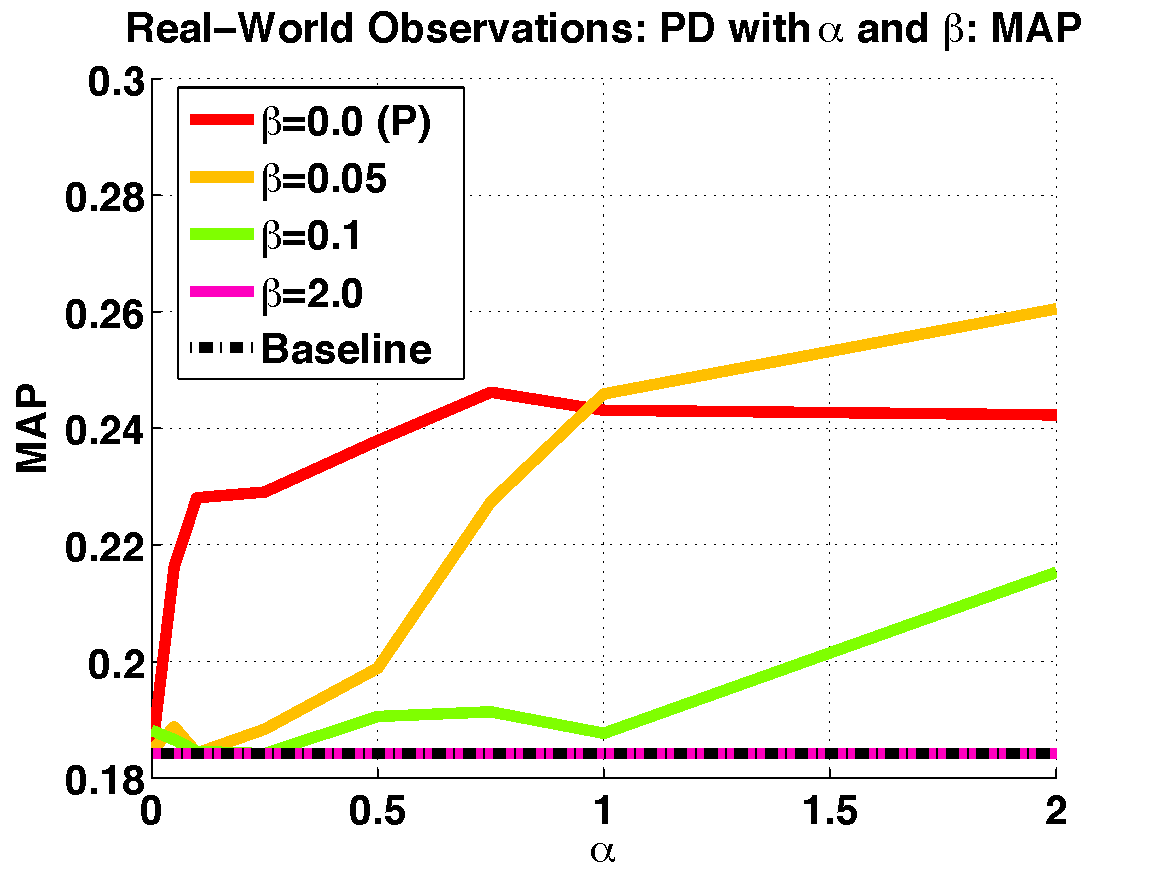
\includegraphics[width=0.5\textwidth]{pics/smucker/pd_map.pdf} & 
		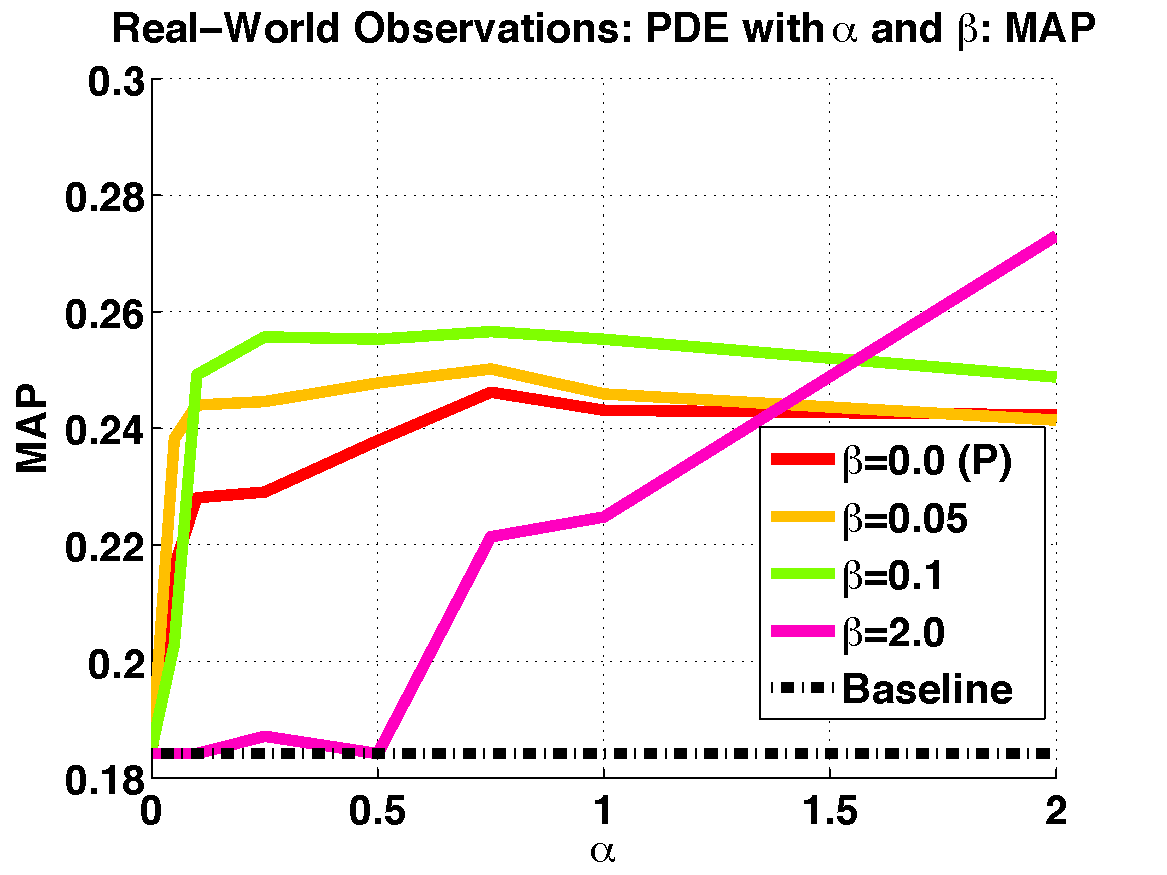
\includegraphics[width=0.5\textwidth]{pics/smucker/pde_map.pdf}
	 \\
		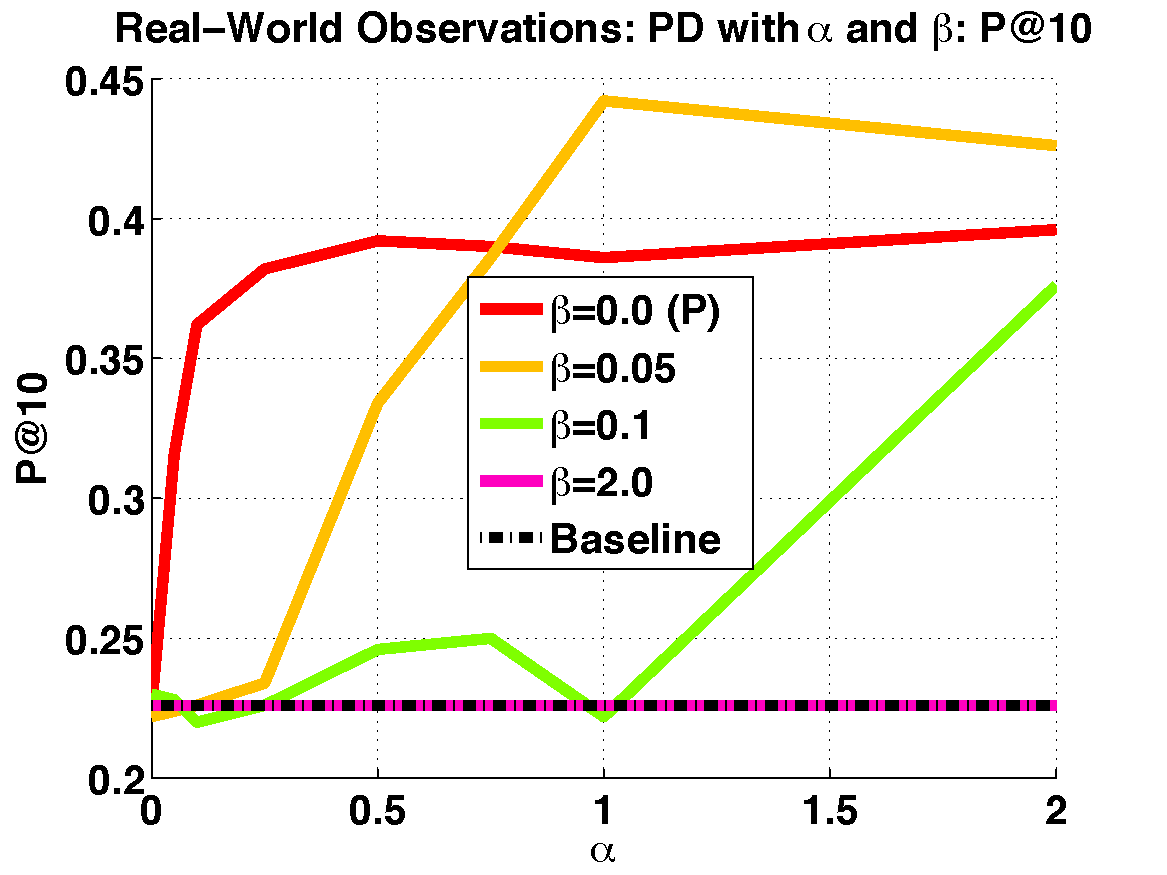
\includegraphics[width=0.5\textwidth]{pics/smucker/pd_p10.pdf} & 
		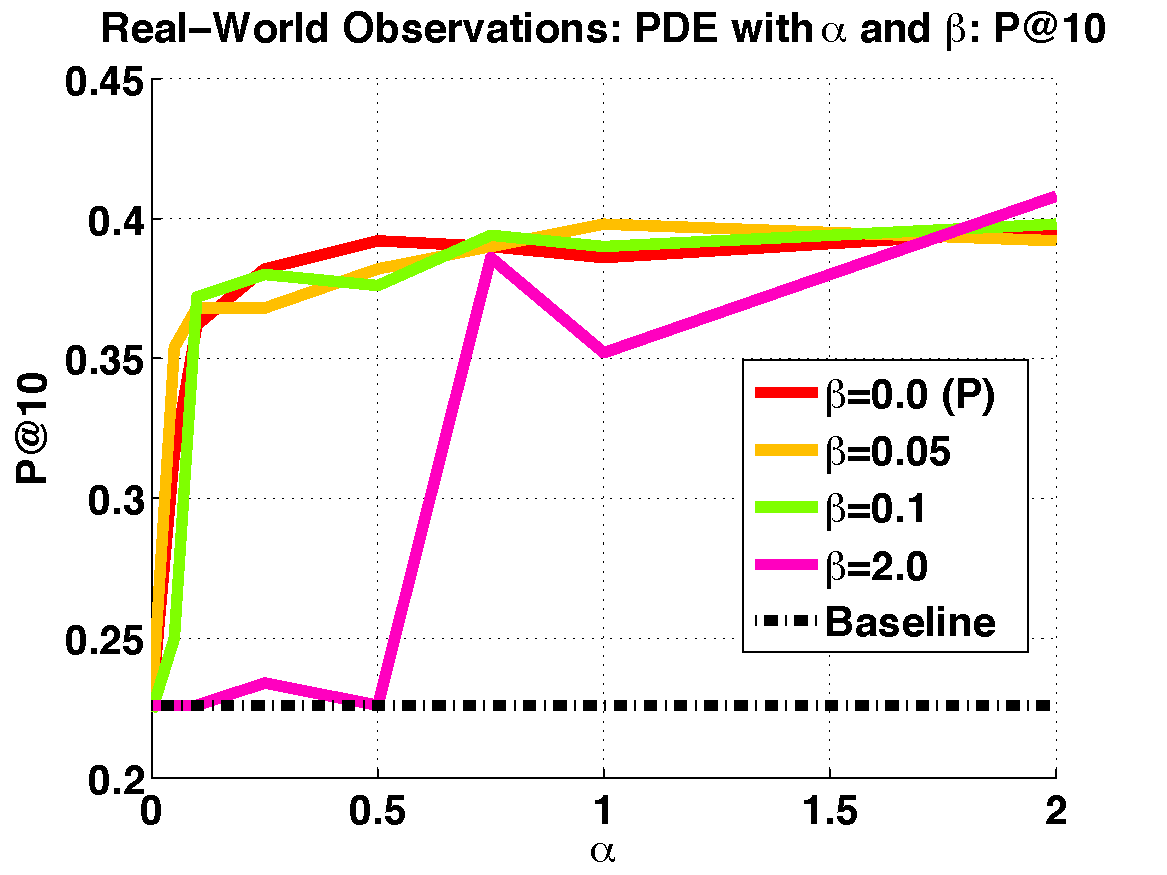
\includegraphics[width=0.5\textwidth]{pics/smucker/pde_p10.pdf}
	\end{array}
	$
	\caption{\textbf{Graphs illustrating performance (MAP and P@10) with variations in $\alpha$ and $\beta$. Graphs show performance for \emph{P} (red line), with variations in $\beta$ values for \emph{PD} and \emph{PDE}.}} \label{fig:noise:graphs}
\end{center}
\end{figure*}